\chapter{Procesamiento Digital de Señales}

\section{Sistemas discretos}

Es necesario convertir una señal análoga a discreta.

\begin{figure}[H]
    \centering
    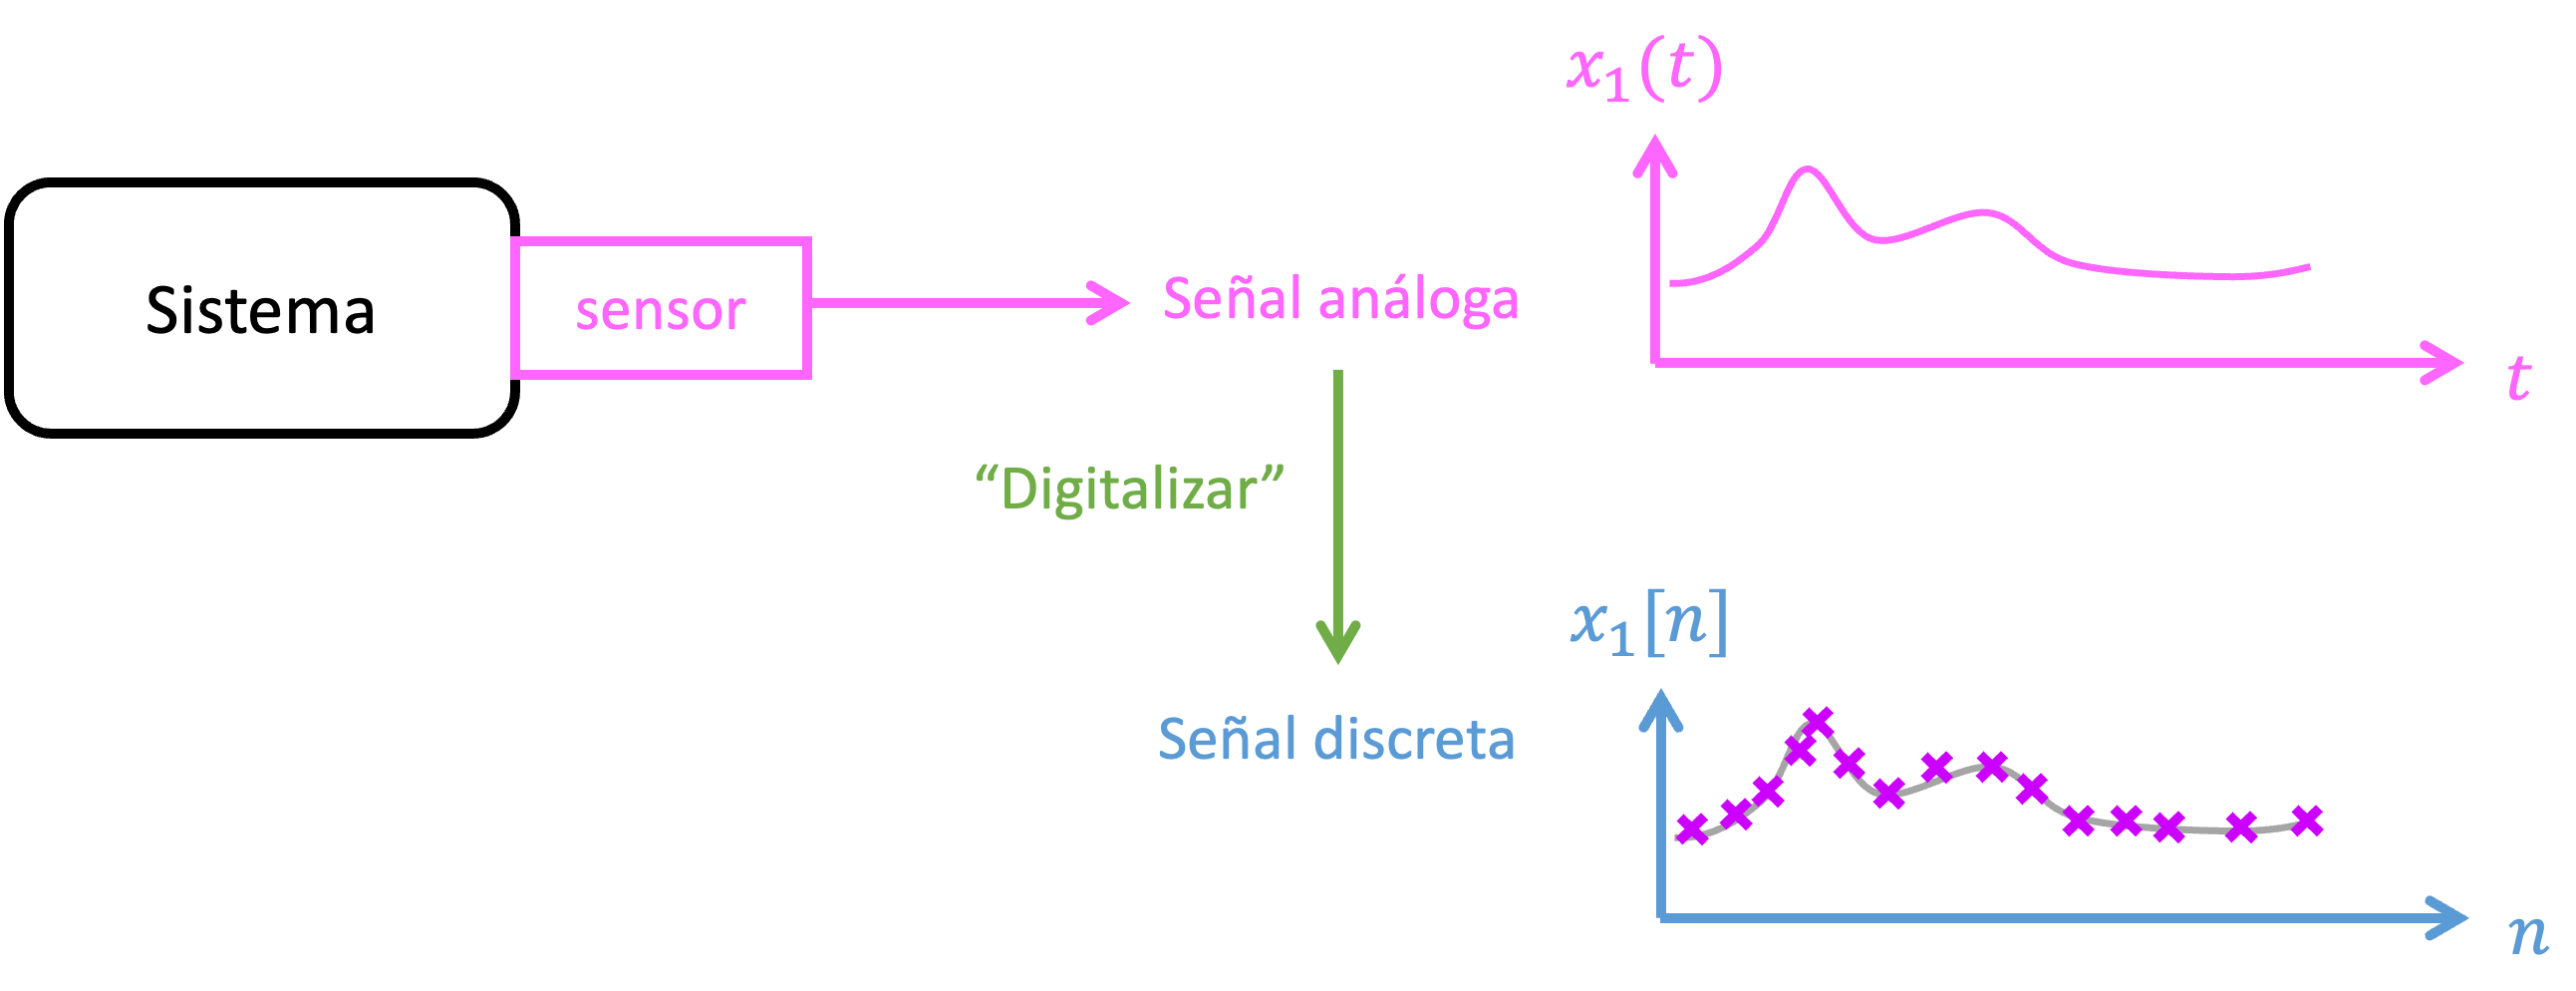
\includegraphics[scale=0.7]{Figuras/sist_discreto.png}
\end{figure}

Razón: Queremos realizar calculos de la señal en un computador.

\begin{figure}[H]
    \centering
    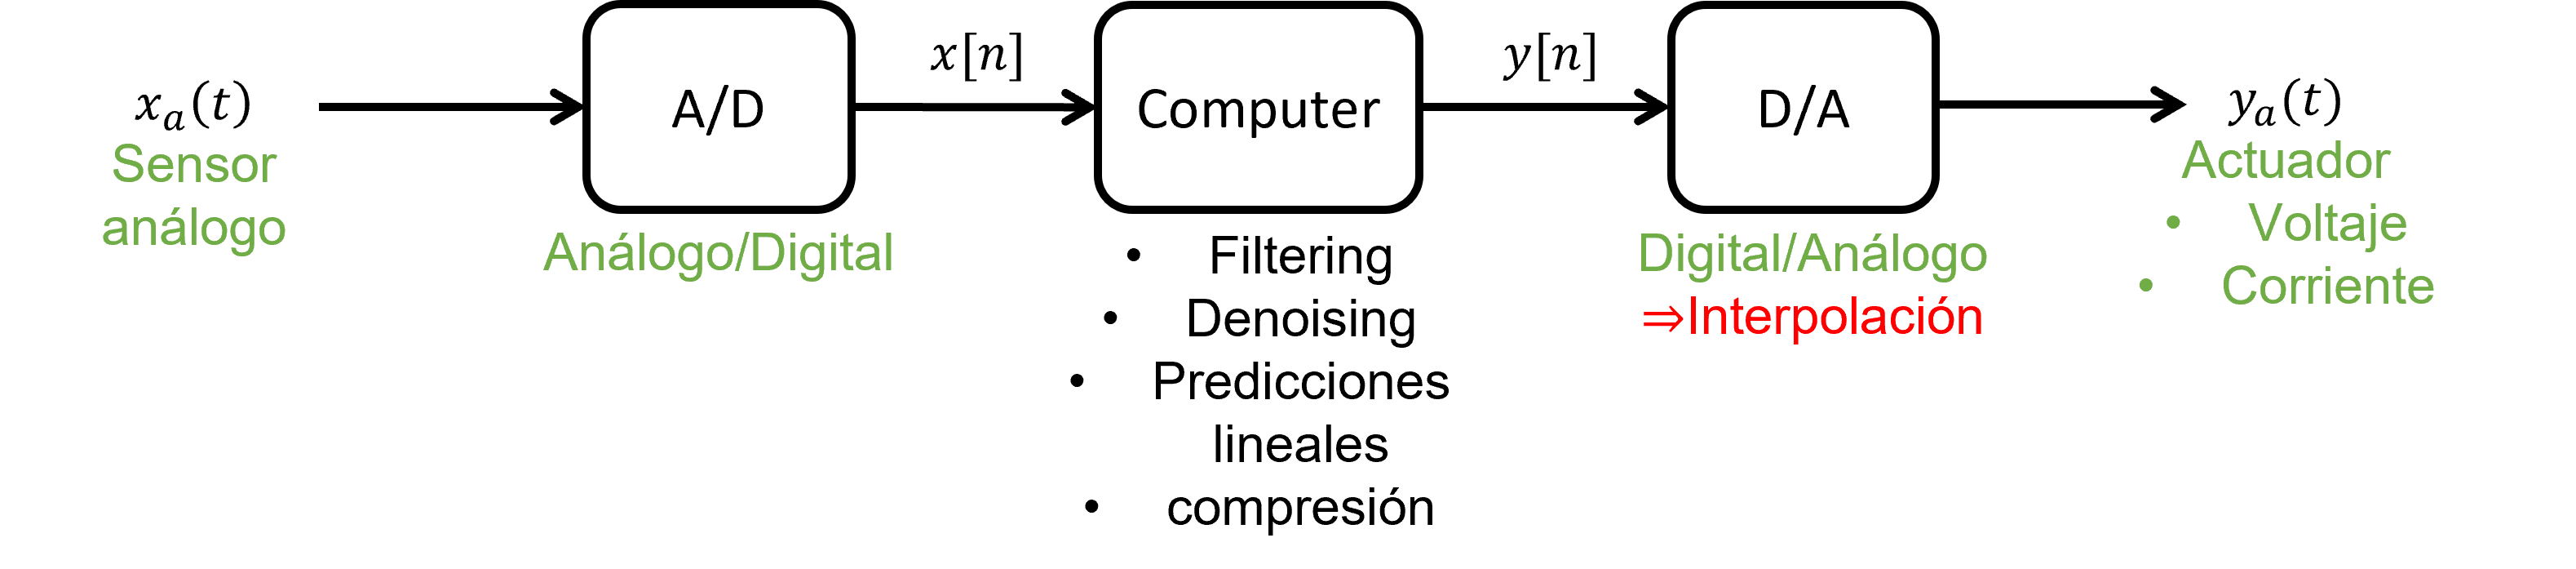
\includegraphics[scale=0.7]{Figuras/sistema_discret.png}
\end{figure}

\subsection{Muestreo}

\begin{enumerate}
    \item Muestreo en el tiempo $\Longrightarrow$ Sampling
    \item Muestreo en amplitud $\Longrightarrow$ Quantization
\end{enumerate}

\subsection{Cuantización}

En el contexto de la conversión analógica a digital (ADC, Analog-to-Digital Conversion), la cuantización (quantization) es el proceso mediante el cual se convierte un valor analógico continuo en un valor digital discreto.

Por ejemplo, una máquina 8 bits $\Longrightarrow$ Números utilizando $2^{8}$ cifras significativas.

\begin{align*}
    \text{Bit} = \left\{ \begin{array}{l}
             0 \\
             1
             \end{array}
   \right. \Longrightarrow 256 \text{ niveles}
\end{align*}

Durante la cuantización, cada valor analógico medido se aproxima al nivel más cercano de entre esos 256 niveles.

Por ejemplo, si el rango es $0 - 5$ V, cada nivel representa un salto de $\Delta = 5/256 \approx 0.0195$ V. Si el valor analógico real es $1.23$ V, el ADC lo “cuantiza” al nivel más cercano, por ejemplo $1.22$ V.

Esta aproximación introduce un error de cuantización, que es la diferencia entre el valor analógico real y el valor cuantizado. Este error es inevitable y depende de la resolución del ADC: a mayor número de bits, menor error de cuantización.

\underline{Nota}: Computadores representan números utilizando dígitos binarios (bits almacenados en flip-flops).\\

\subsection{Señal en tiempo discreto}

\begin{figure}[H]
    \centering
    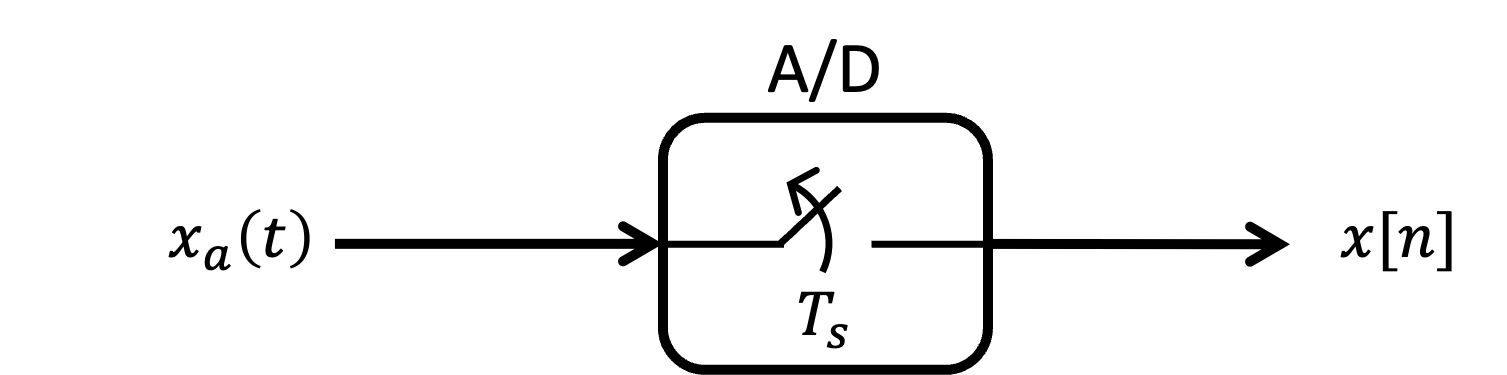
\includegraphics[scale=0.7]{Figuras/AD.png}
\end{figure}


\begin{align*}
    x[n]=x_a(nT_s)
\end{align*}

\noindent donde $x[n]$ es la señal en tiempo discreto, $T_s$ es el paso temporal de muestreo, y $n$ es el índice temporal (número entero).\\

\begin{figure}[H]
    \centering
    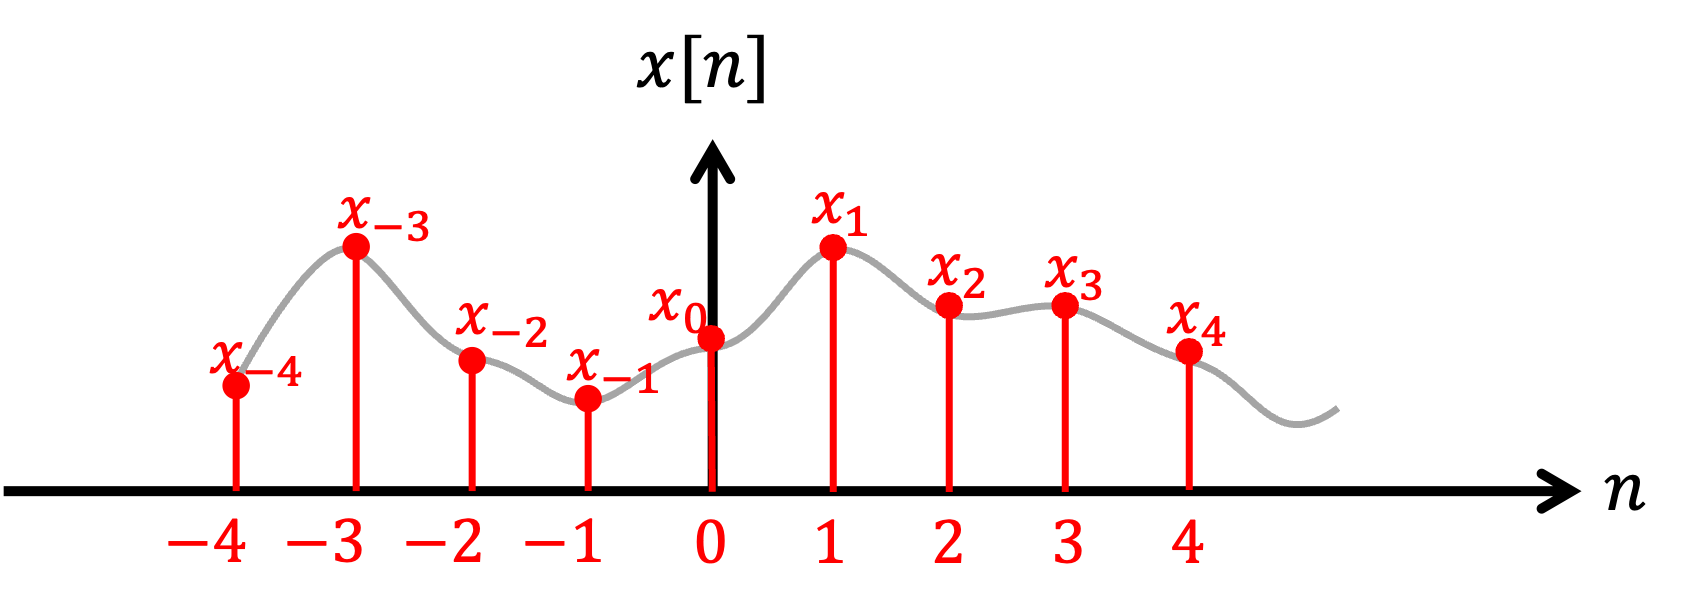
\includegraphics[width=4in]{Figuras/senaldiscreta.png}
\end{figure}

La representación matemática del muestreo se puede realizar utilizando la \underline{Función pulso unitario}:

\begin{figure}[H]
    \centering
    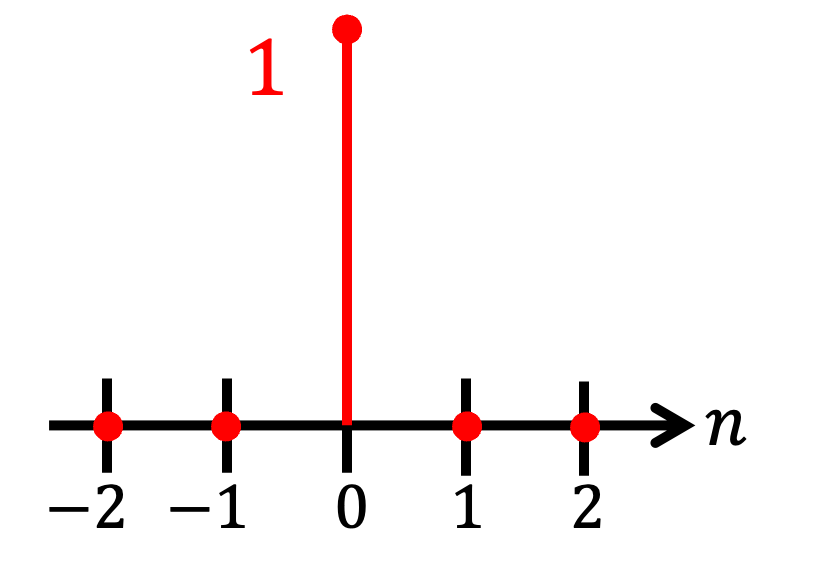
\includegraphics[scale=0.7]{Figuras/pulso_unitario.png}
\end{figure}

\begin{align*}
    \delta[n] = 
    \begin{cases}
        1, & n=0\\
        0,& n \neq 0
    \end{cases}
\end{align*}

\begin{align*}
    x[n]=\sum_{k=0}^{N-1} x_k \delta[n-k]=x_0\delta[n]+x_1\delta[n-1]+x_2\delta[n-2]+...+x_{N-1}\delta[n-(N-1)]
\end{align*}

\begin{align*}
    \{x_n\}_0^{N-1}=\{x_0,x_1,x_2,...,x_{N-1}\} \Longrightarrow \text{Arreglo de N puntos (vector)}
\end{align*}


\section{Análisis en frecuencia}

\begin{figure}[H]
    \centering
    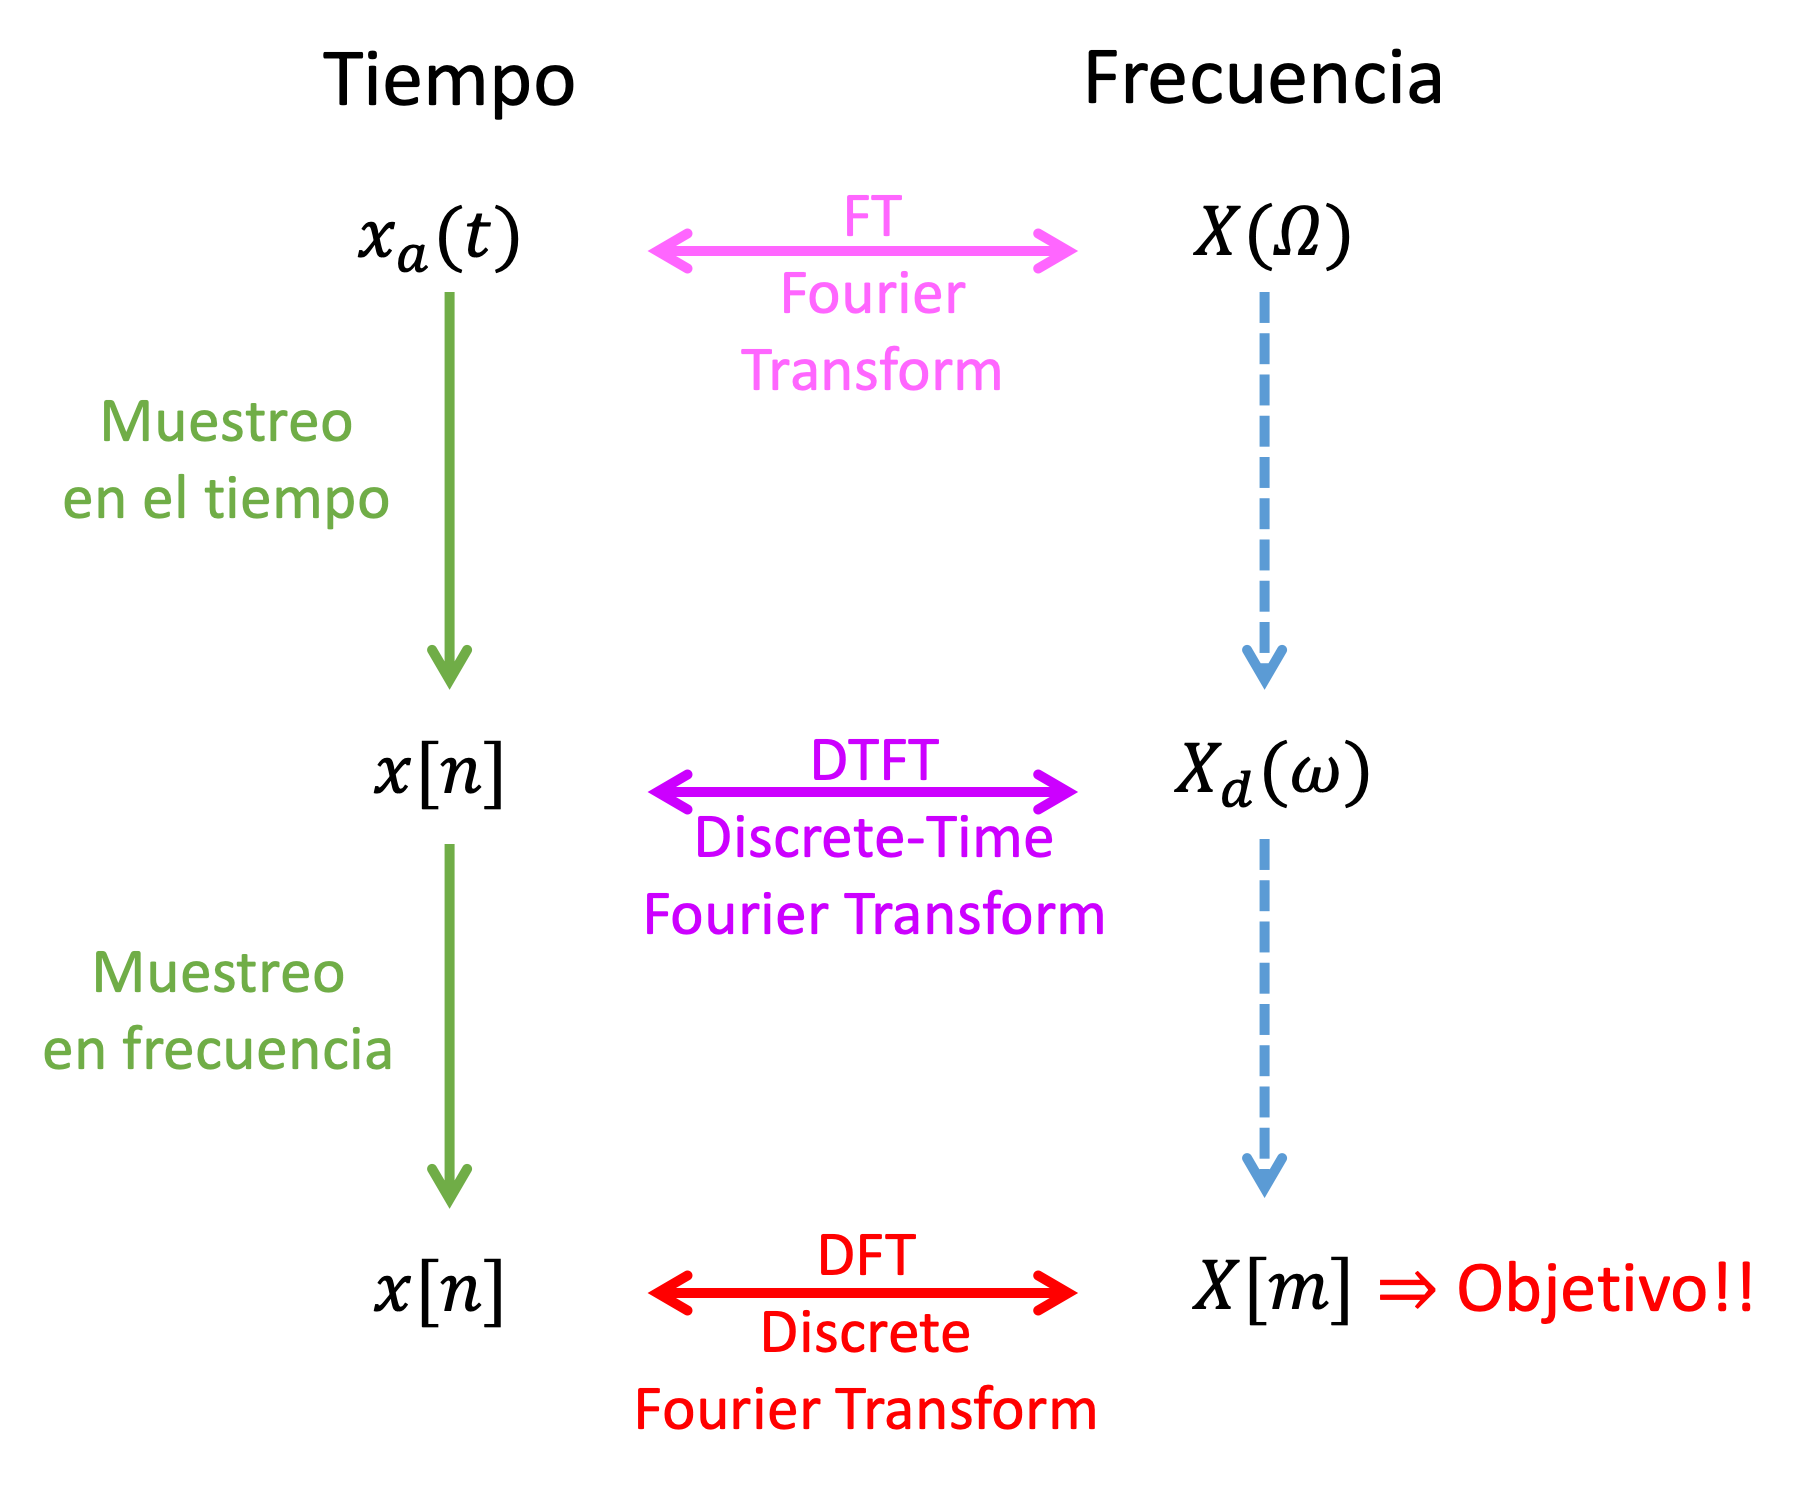
\includegraphics[scale=0.7]{Figuras/analisis_frec.png}
\end{figure}

\noindent \emph{Nota:} $j = \sqrt{-1}$ es el número complejo.\\

\subsection{Continuous-Time Fourier Transform (CTFT)}

\begin{align*}
    X(\Omega) &= \int_{-\infty}^{+\infty}x_a(t)e^{-j\Omega t}dt \quad \text{(CTFT)}\\
    x_a(t) &= \frac{1}{2\pi}\int_{-\infty}^{+\infty}X(\Omega)e^{+j\Omega t}d\Omega \quad \text{(inverse CTFT)}
\end{align*}

$t, \Omega \in \mathbb{R}$, $x_a(t)\in \mathbb{R}$, $X(\Omega)\in \mathbb{C}$\\

\subsection{Discrete-time Fourier Transform (DTFT)}

Supongamos que la señal $x(t)$ es discretizada en el tiempo, $x[n] = x(n T_s)$, donde $T_s$ es el período de muestreo. Entonces, el DTFT se define:

\begin{align*}
    X_d(\omega) &= \sum_{n=-\infty}^{\infty}x[n]e^{-j\omega n} \quad \text{(DTFT)}\\
    x[n] &= \frac{1}{2\pi}\int_{-\infty}^{\infty}X_d(\omega)e^{+j\omega n}d\omega \quad \text{(inverse DTFT)}
\end{align*}

donde $\omega \in \mathbb{R}$, $n \in \mathbb{Z}$.

\subsection{Discrete Fourier Transform (DFT)}

La DFT opera sobre una secuencia de $N$ puntos en tiempo, $x[n], n \in \{0,1,2,\ldots,N-1\}$, y produce una secuencia de $N$ puntos en frecuencia, $X[m], m \in \{0,1,2,\ldots,N-1\}$.

\begin{align*}
    X[m] &= \sum_{n=0}^{N-1} x_ne^{-j\frac{2\pi}{N}nm} \quad \text{(DFT)}\\
    x[n] &= \frac{1}{N}\sum_{m=0}^{N-1}X_me^{+j\frac{2\pi}{N}nm} \quad \text{(Inverse DFT)}
\end{align*}

donde $n,m \in \{0,1,2,\ldots,N-1\}$.\\

\emph{Nota 1}: Se asume que la secuencia $x[n]$ es periódica.\\

\emph{Nota 2}: Fast Fourier Transform (FFT) es un algoritmo computacional para calcular el DFT.\\

\subsection{Relación entre DFT y DTFT}

\begin{align*}
    X[m]=X_d(\omega)\bigg|_{\omega=\frac{2\pi}{N}m}
\end{align*}

\subsection{Relación entre DTFT y CTFT}

\begin{align*}
    X_d(\omega) = \frac{1}{T} \sum_{l=-\infty}^{+\infty} X \left(\underbrace{\frac{\omega + 2\pi l}{T}}_{= \Omega} \right)
\end{align*}

\section{Criterio de muestreo de Nyquist}

En DSP, queremos muestrear la señal sin pérdida de información (``lossless''). Entonces, hay que elegir correctamente el intervalo de muestreo $T_s$ (sampling time).\\

\begin{theorem}[Teorema de Nyquist]
    La frecuencia de muestreo de una señal digital debe ser al menos el doble de la máxima frecuencia de la señal análoga:
    $$F_s > 2 f_{\max}$$
\end{theorem}

\section{Aliasing}

Aliasing es un fenómeno que ocure cuando el terorema de Nyquist no se cumple, es decir, $F_s \leq 2 f_{\max}$. Ocurre cuando una señal análoga no puede ser reconstruida por la señal digitalizada.\\

\underline{Ejemplo}: Video del ``helicoptero mágico'' \url{https://www.chrisfay.de/helicopter-video}. 

\subsection{Aliasing en dominio del tiempo}

\begin{figure}[H]
    \centering
    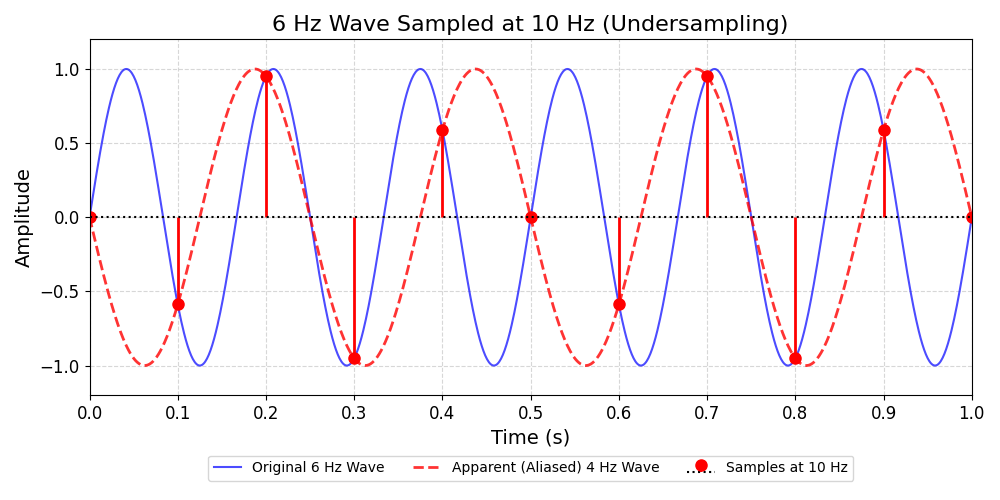
\includegraphics[width=6in]{Figuras/AliasingTimeExample.png}
\end{figure}

\subsection{Aliasing en dominio de frecuencia}

\begin{figure}[H]
    \centering
    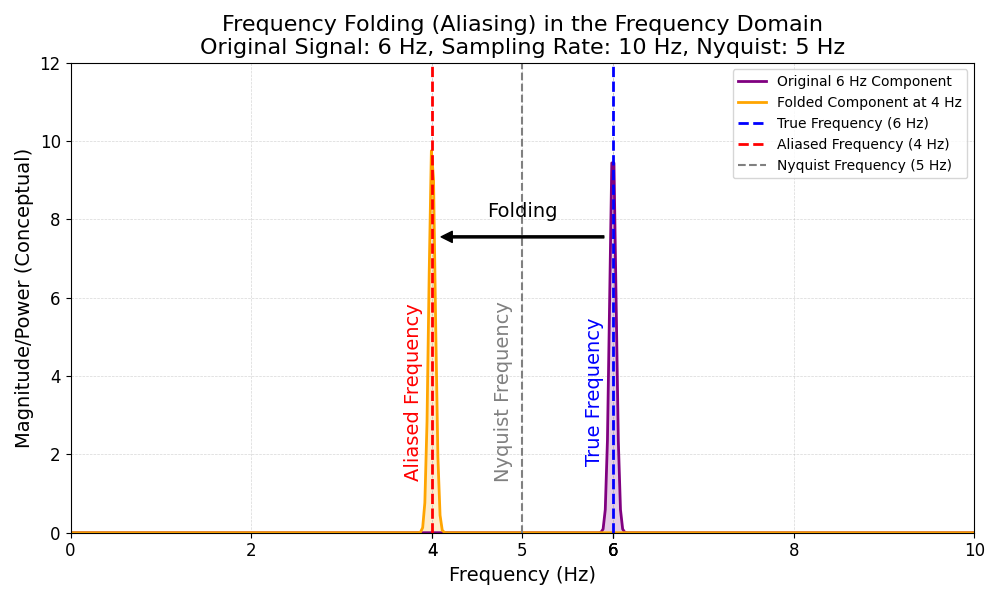
\includegraphics[width=6in]{Figuras/aliasing_frequency_folding.png}
\end{figure}

Considere $f = 2 \pi \Omega$, donde $f$ es frecuencia [Hz] y $\Omega$ es frecuencia (cicular) [rad/s].

\subsubsection{Sin Aliasing}

\begin{figure}[H]
\centering
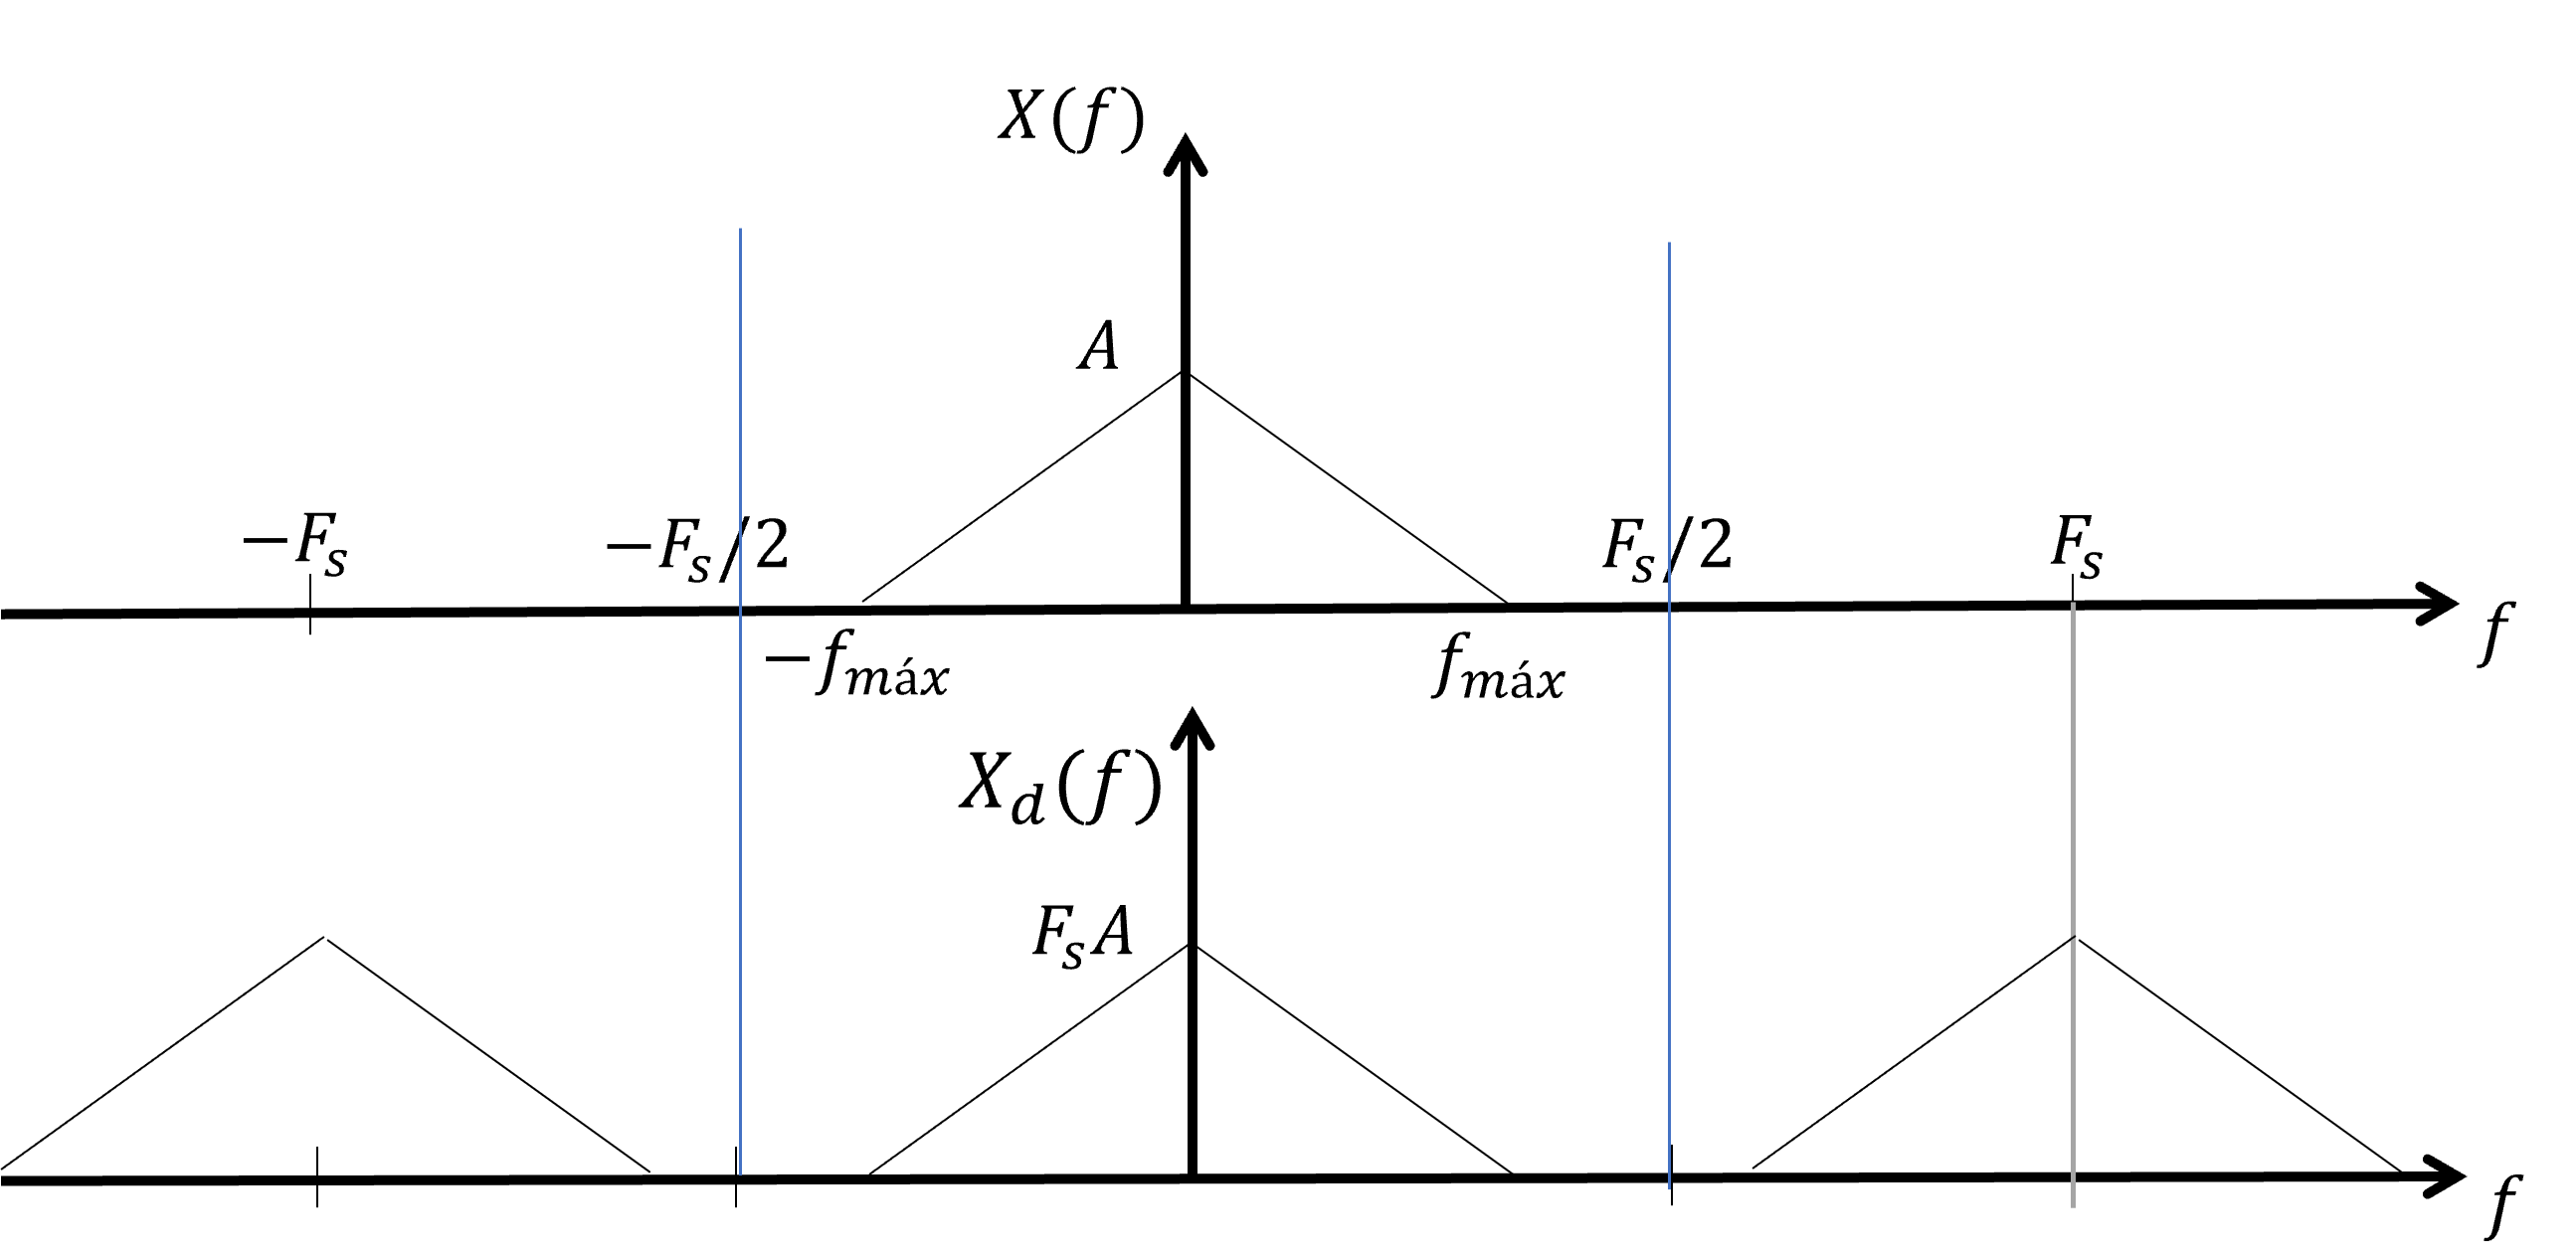
\includegraphics[scale=0.7]{Figuras/sin_aliasing.png}
\end{figure}

\begin{align*}
    F_s &> 2f_{max}\\
    f_{max} &< \frac{F_s}{2}=F_N \quad \text{(frecuencia de Nyquist)}
\end{align*}

\subsubsection{Con Aliasing}

\begin{figure}[H]
\centering
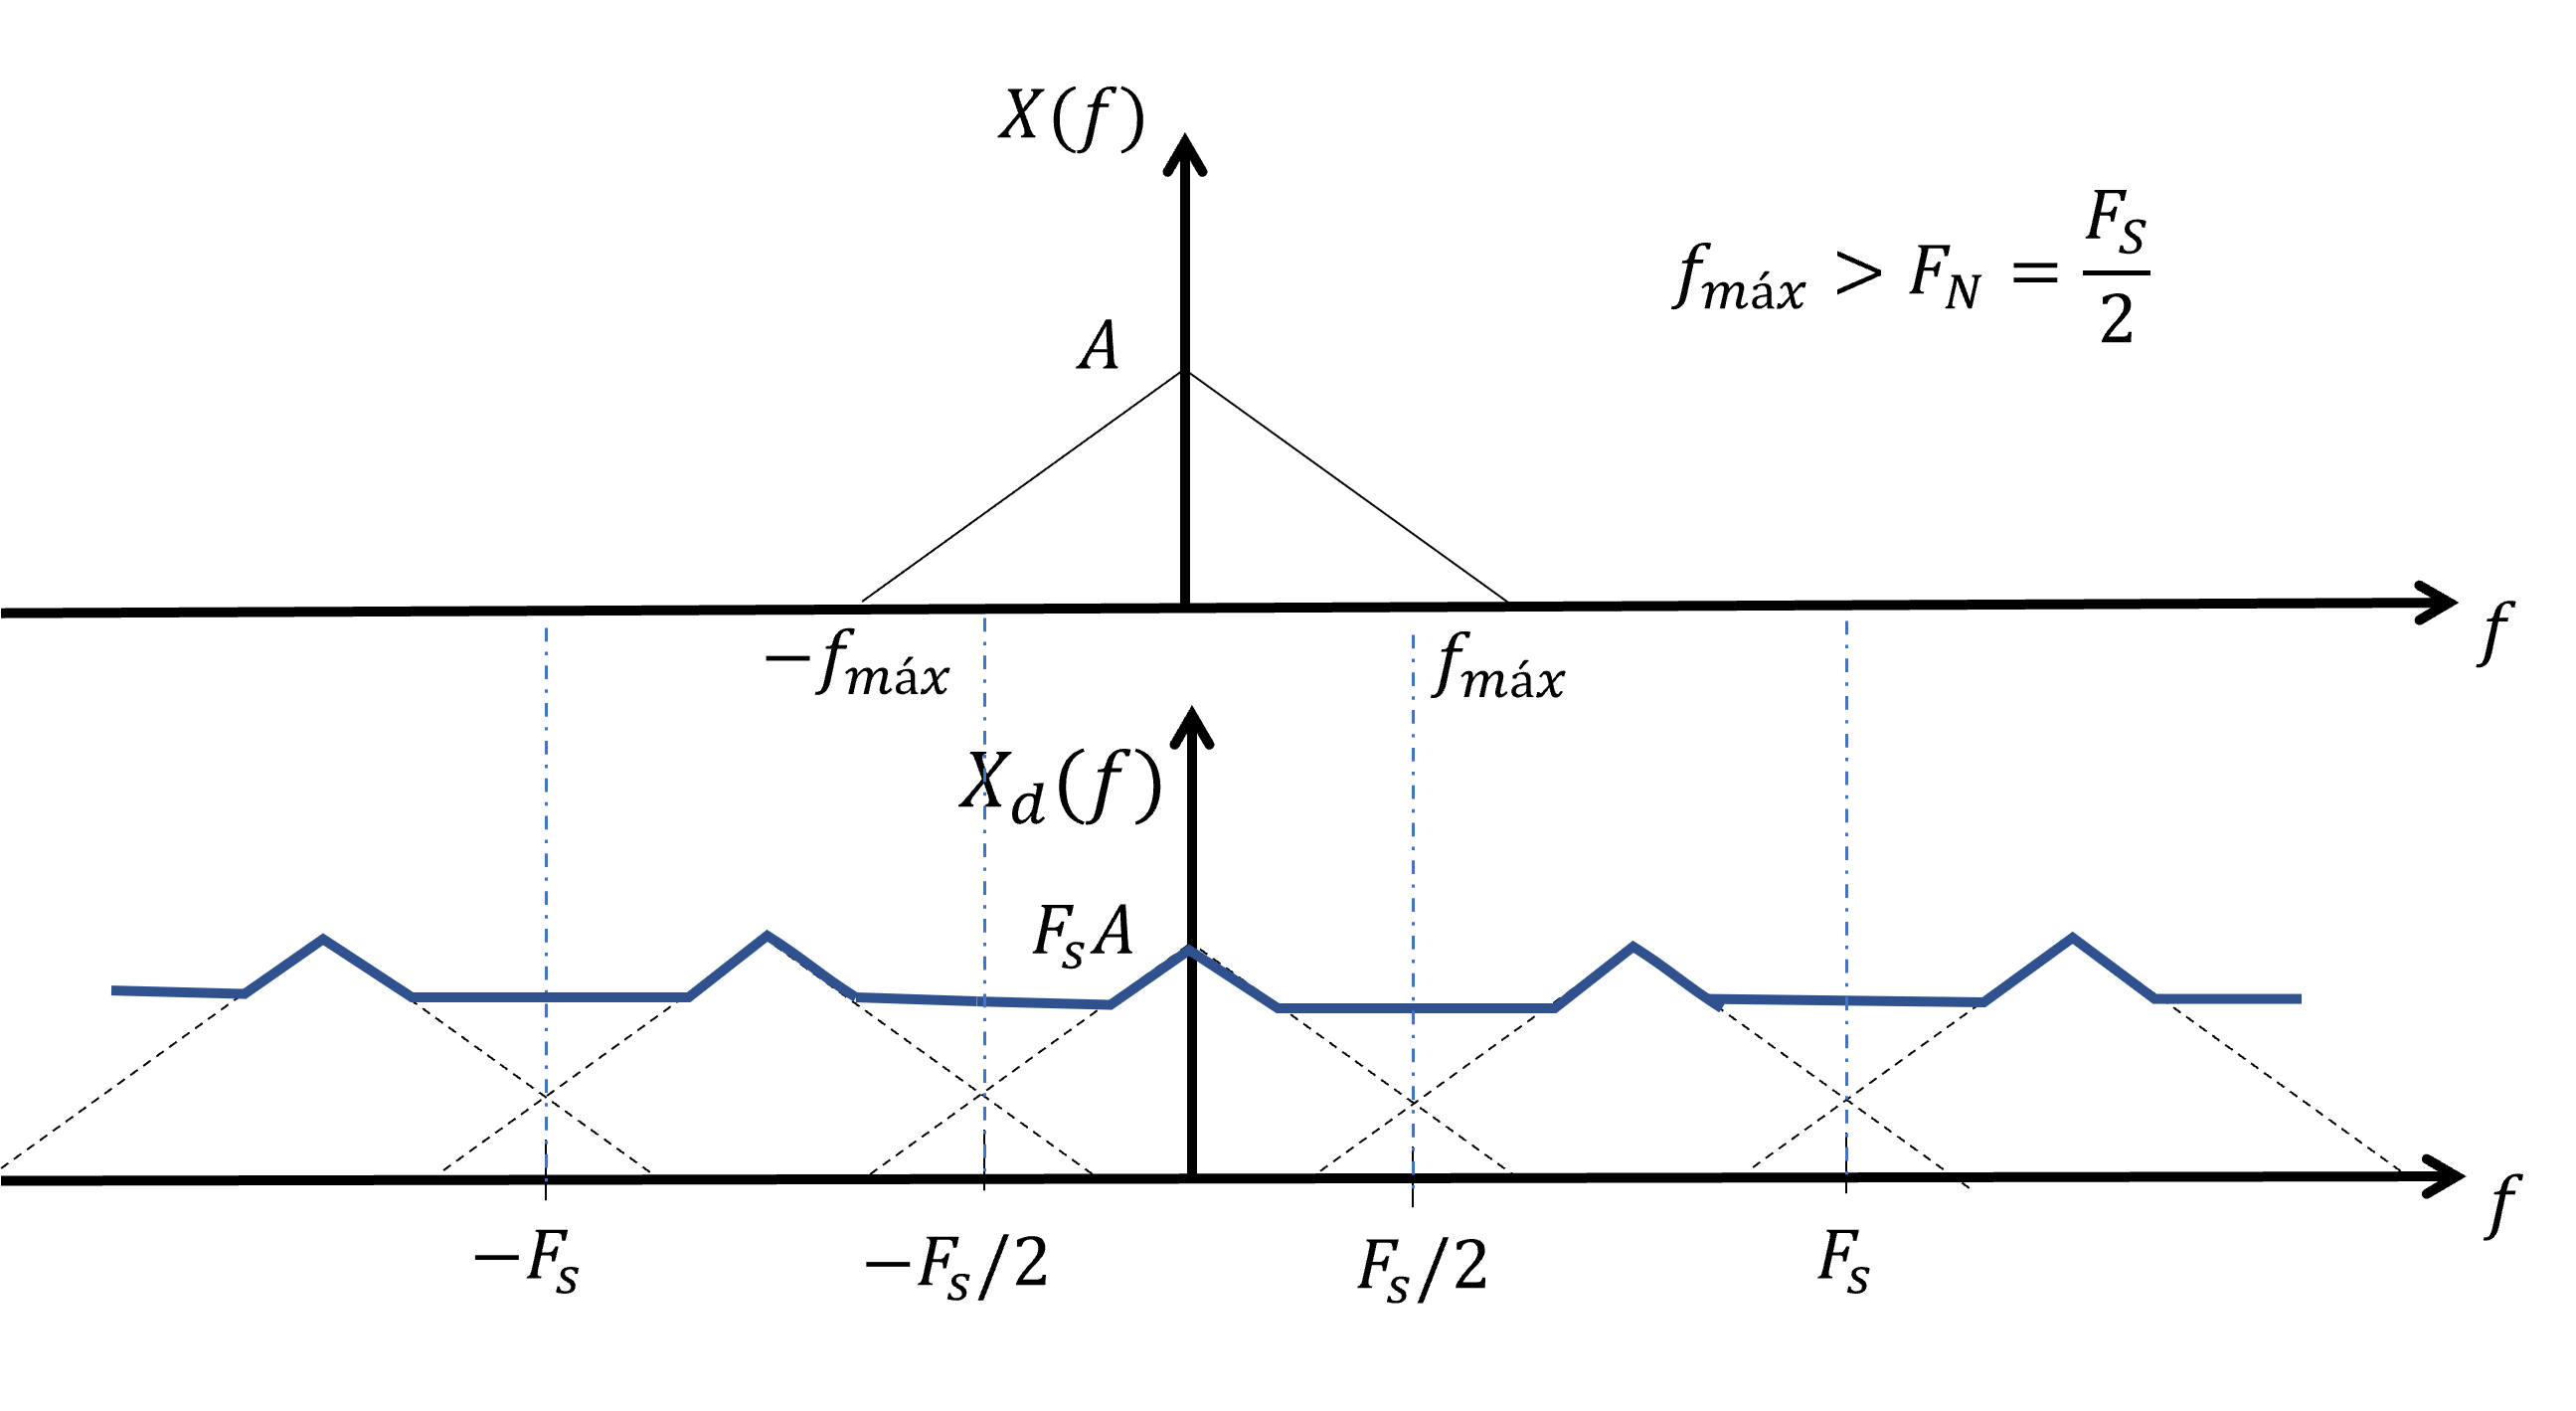
\includegraphics[scale=0.7]{Figuras/con_aliasing.png}
\end{figure}

Ejemplo: PSD de respuesta estructural de un sistema 3DOF

\begin{figure}[H]
\centering
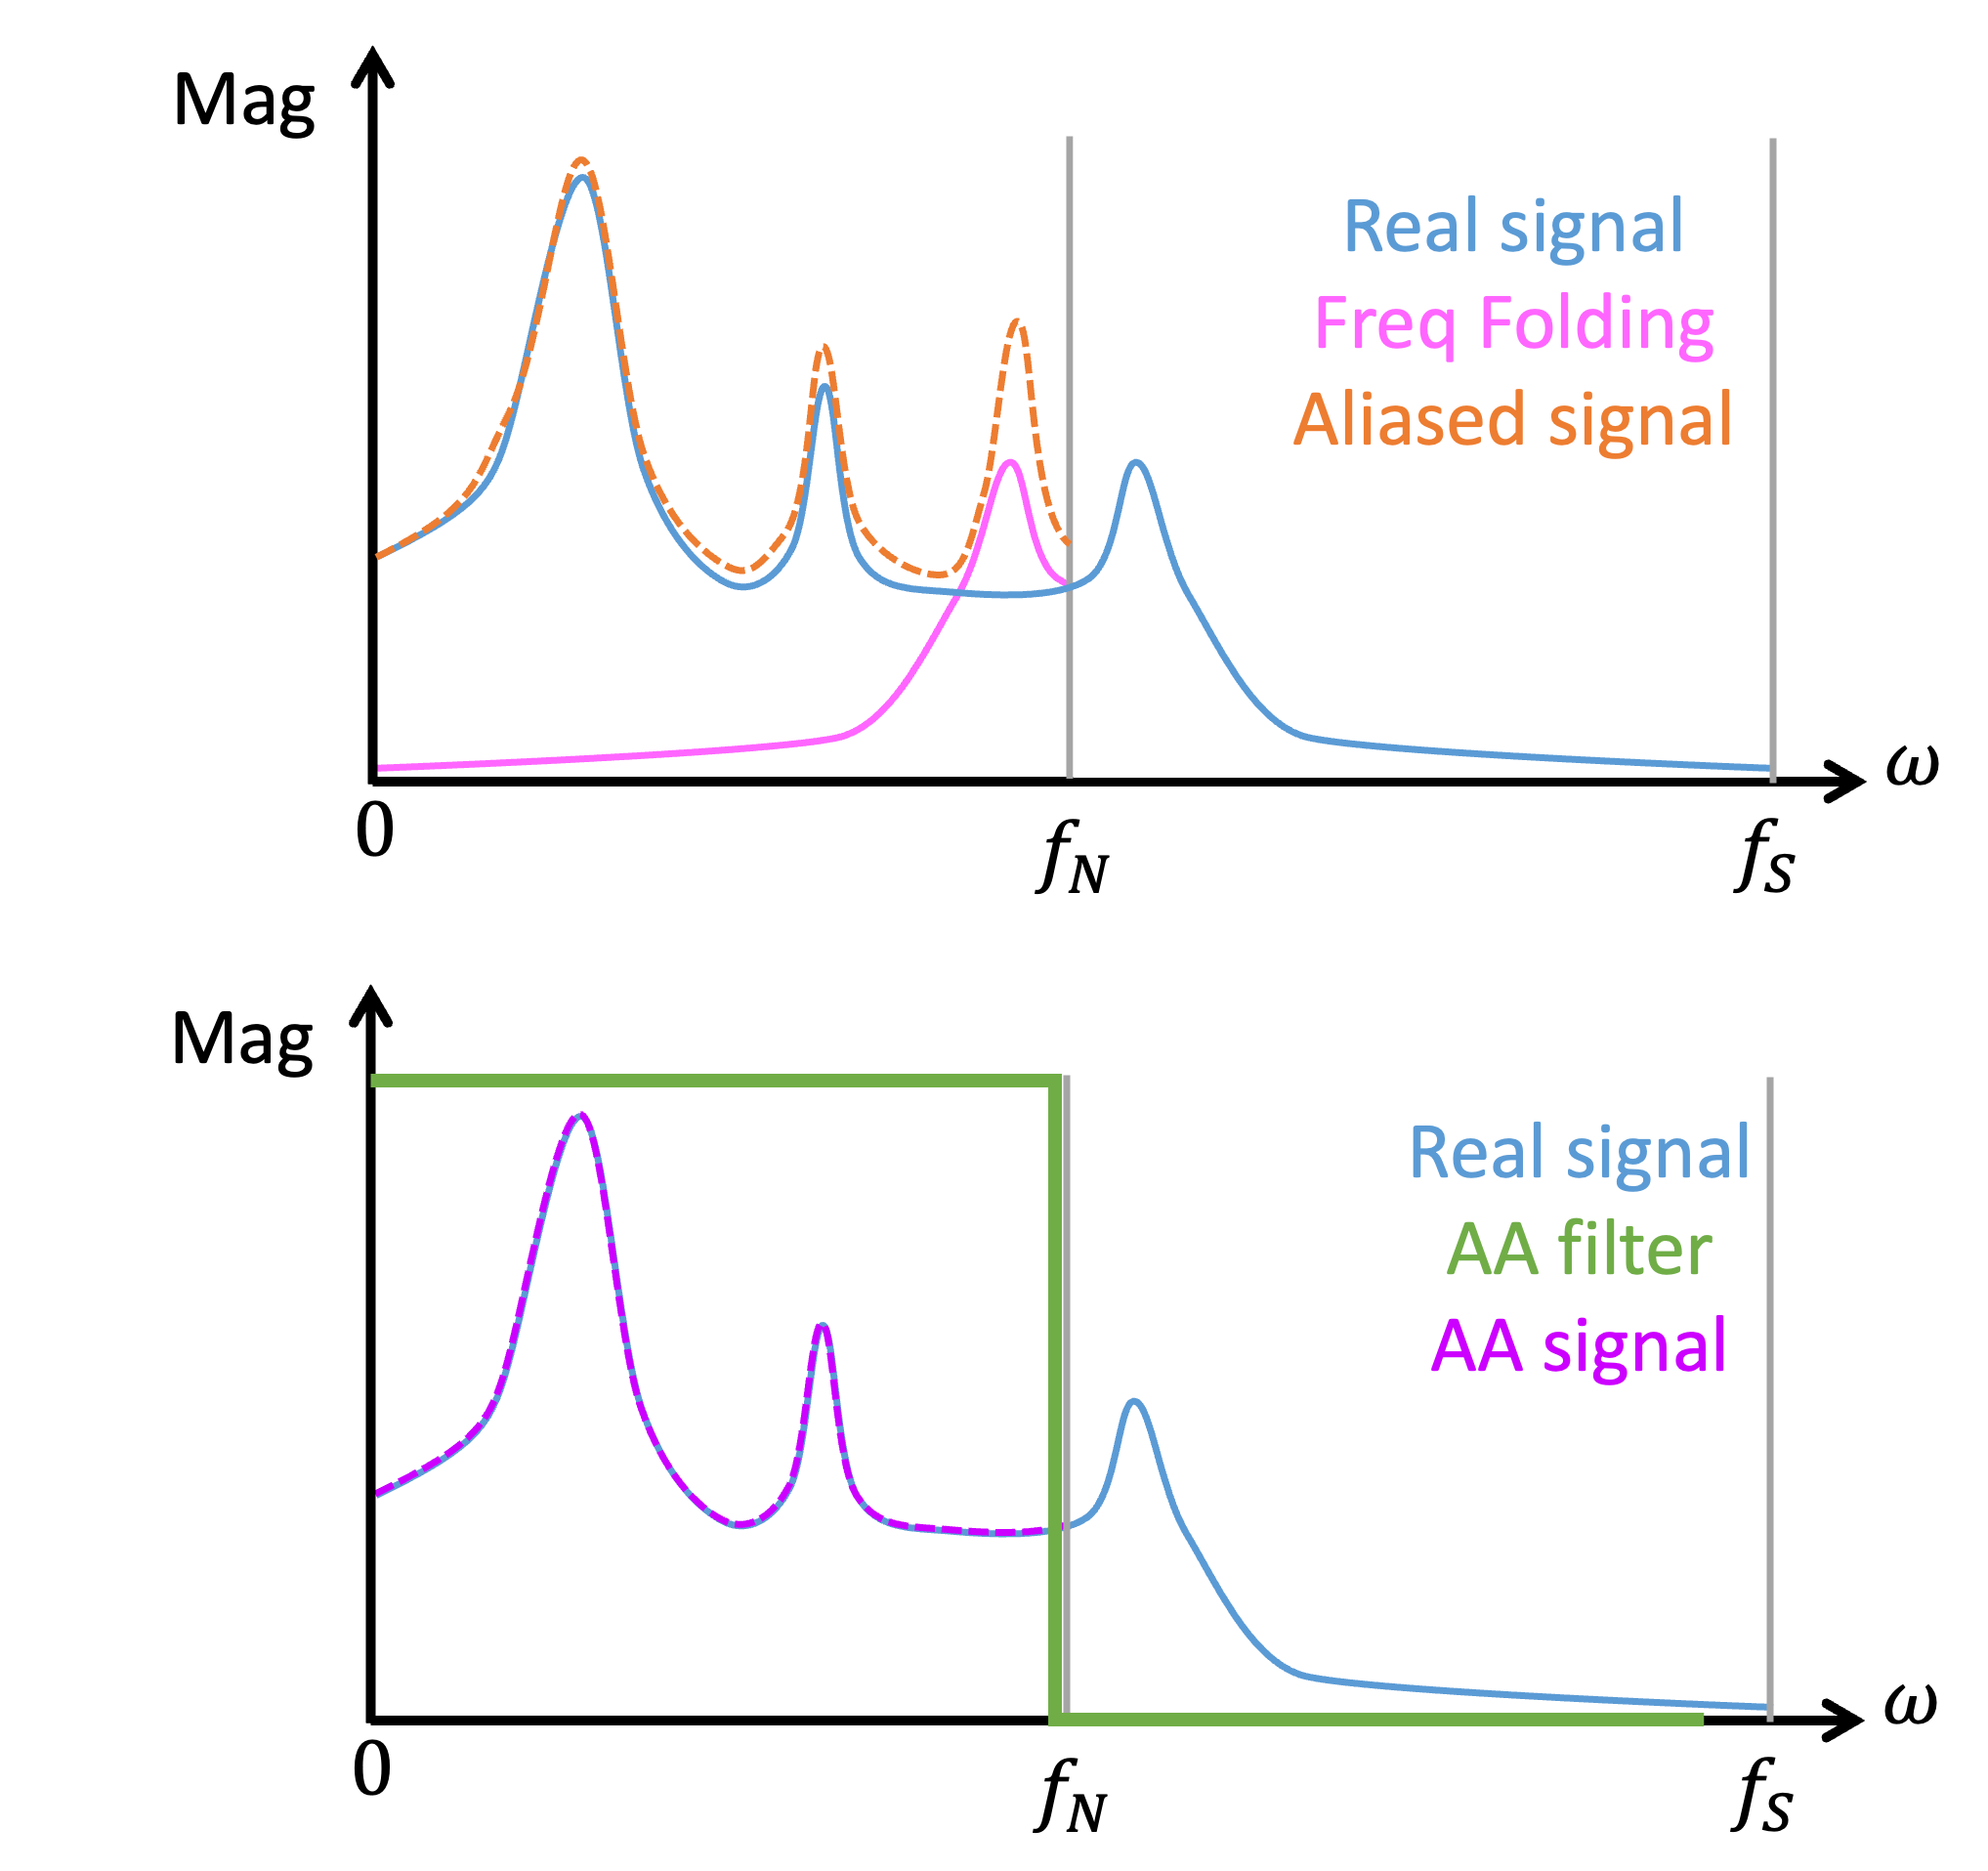
\includegraphics[width=5in]{Figuras/AAexample.png}
\end{figure}

\begin{itemize}
    \item Filtro anti-aliasing (AA) de paso bajo (low-pass) es utilizado para eliminar el ``aliasing'' de la respuesta en frecuencia.
    \item Filtro AA tiene que ser aplicado antes del muestreo en el tiempo.
\end{itemize}

\begin{figure}[H]
\centering
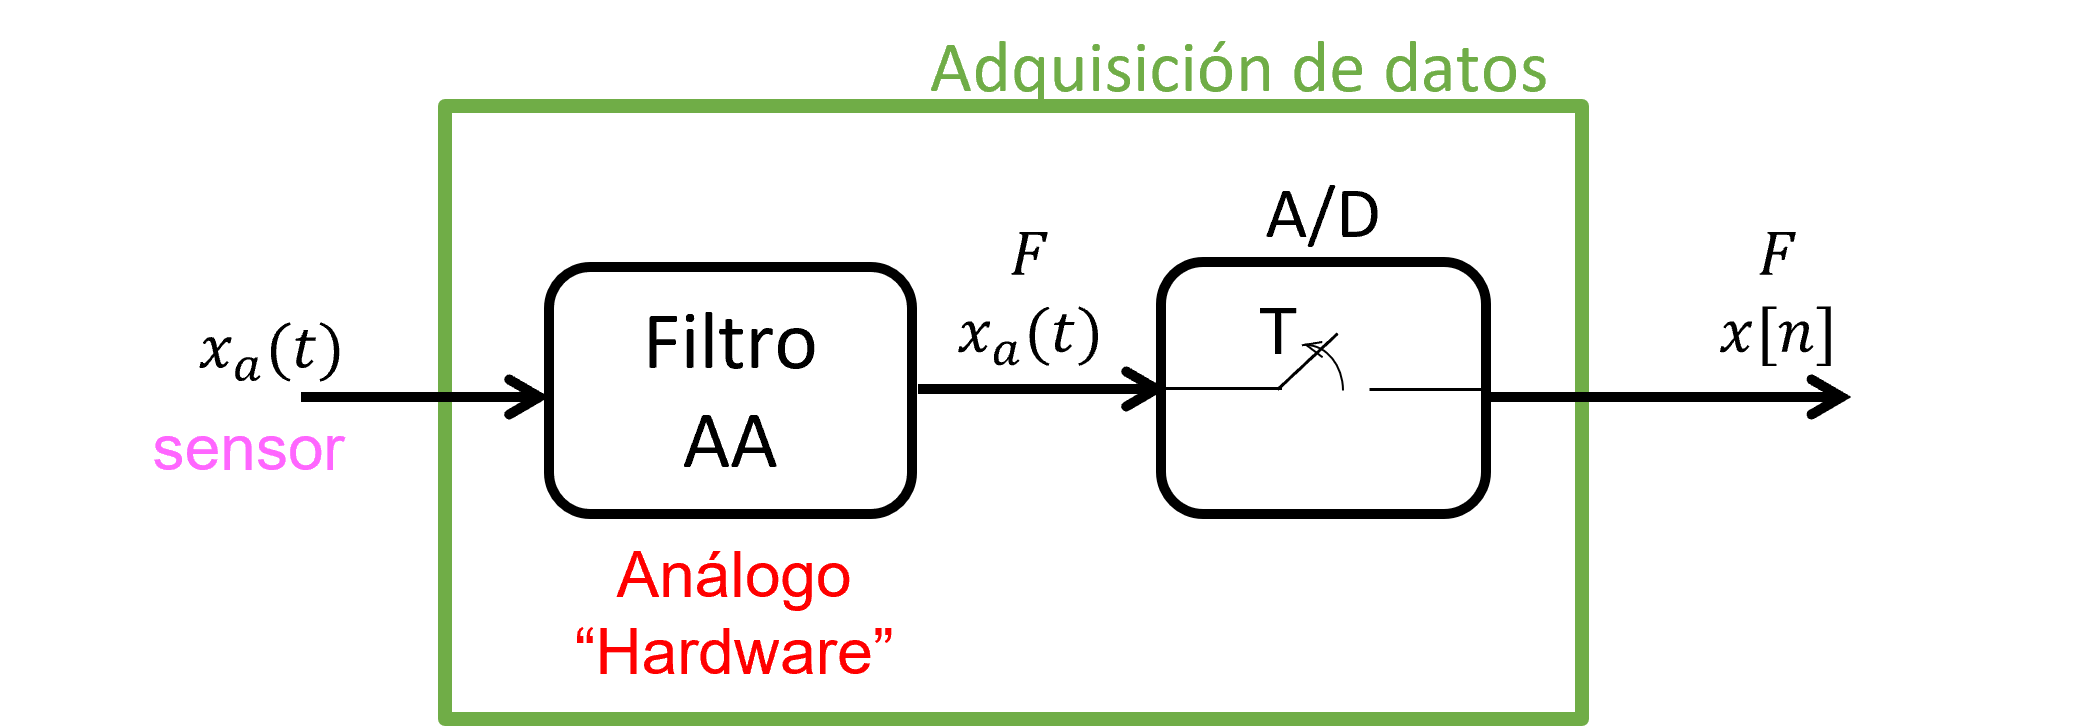
\includegraphics[scale=0.7]{Figuras/filtroAA2.png}
\end{figure}

\subsection{Spectral Leakage}
CTFT/DTFT/DFT asumen que la \underline{señal es periódica}, es decir, que la señal se repite luego de un periodo $T_1$ indefinidamente.
$$ x(t) = x(t+nT_1) $$
Si la señal no es periódica, ocurren saltos abruptos.
\begin{figure}[H]
\centering
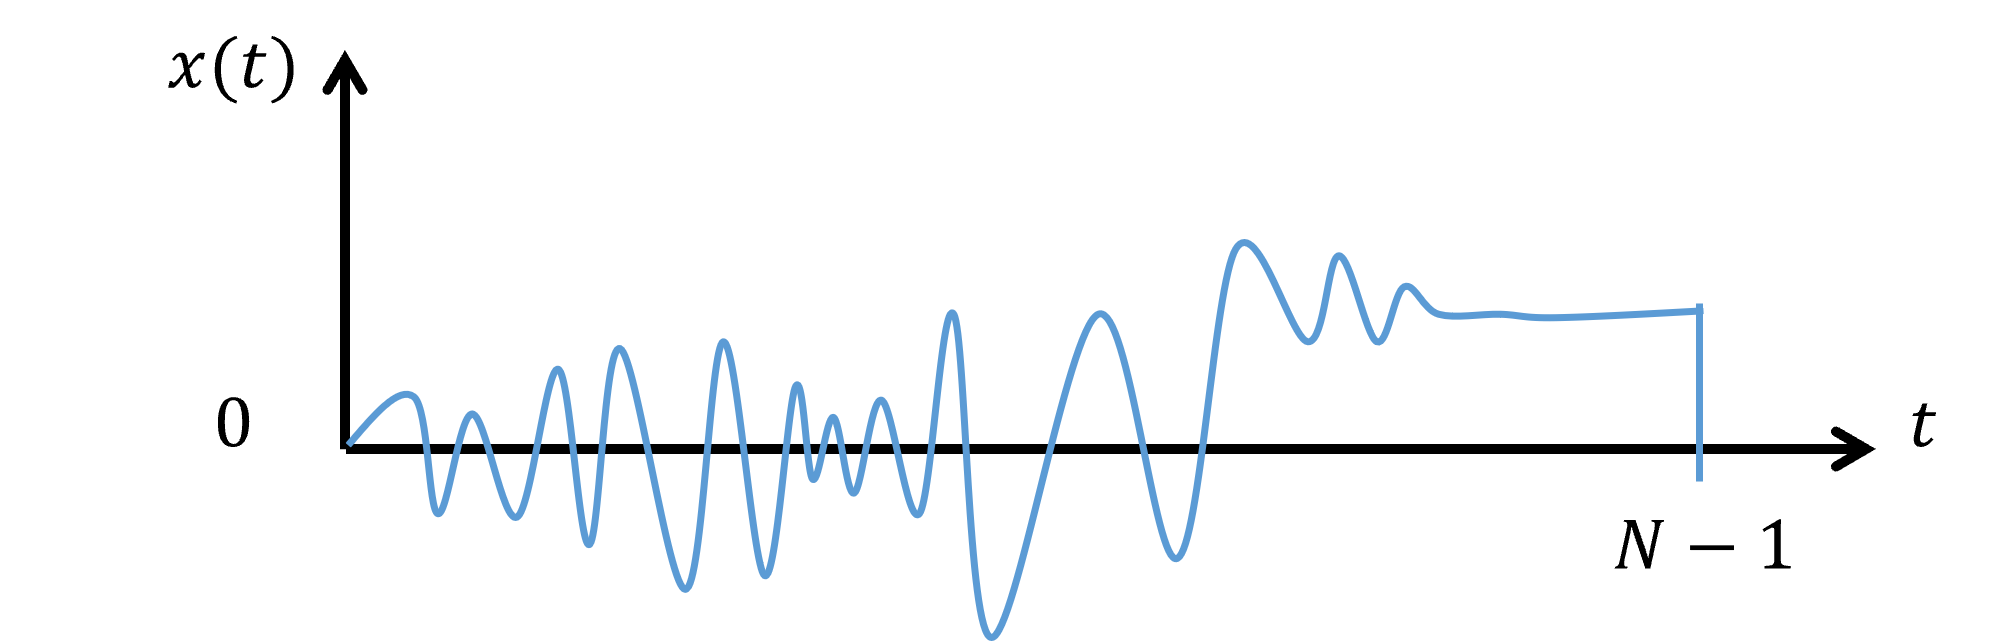
\includegraphics[scale=0.7]{Figuras/FT.png}
\end{figure}

\begin{figure}[H]
\centering
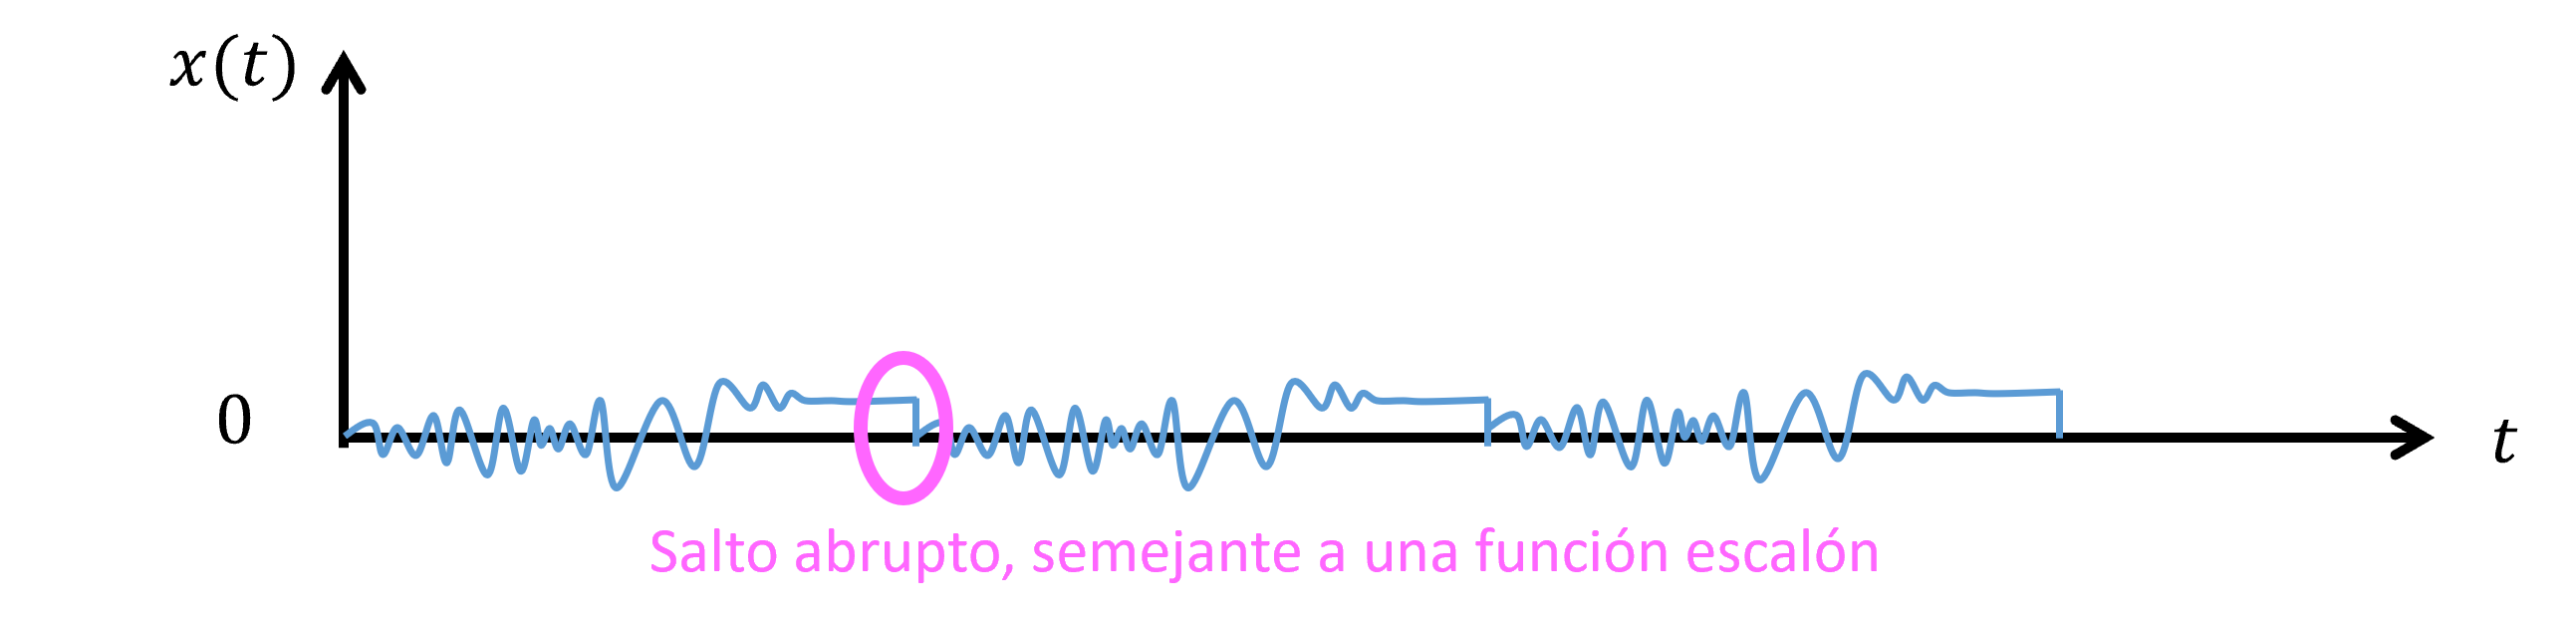
\includegraphics[scale=0.6]{Figuras/DFT.png}
\end{figure}

Este salto abrupto es semejante a una función escalón. Recordar que una función escalón se puede escribir como una Serie de Fourier que es una suma de armónicas con distinta frecuencia. Por lo tanto, al calcular $X[m]$ (DFT de $x[n]$) surge el fenómeno de ``spectral leakage'', donde se agregan armónicas artificiales producto del escalón generado.\\
\par \underline{Ejemplo}:

\begin{figure}[H]
    \centering
    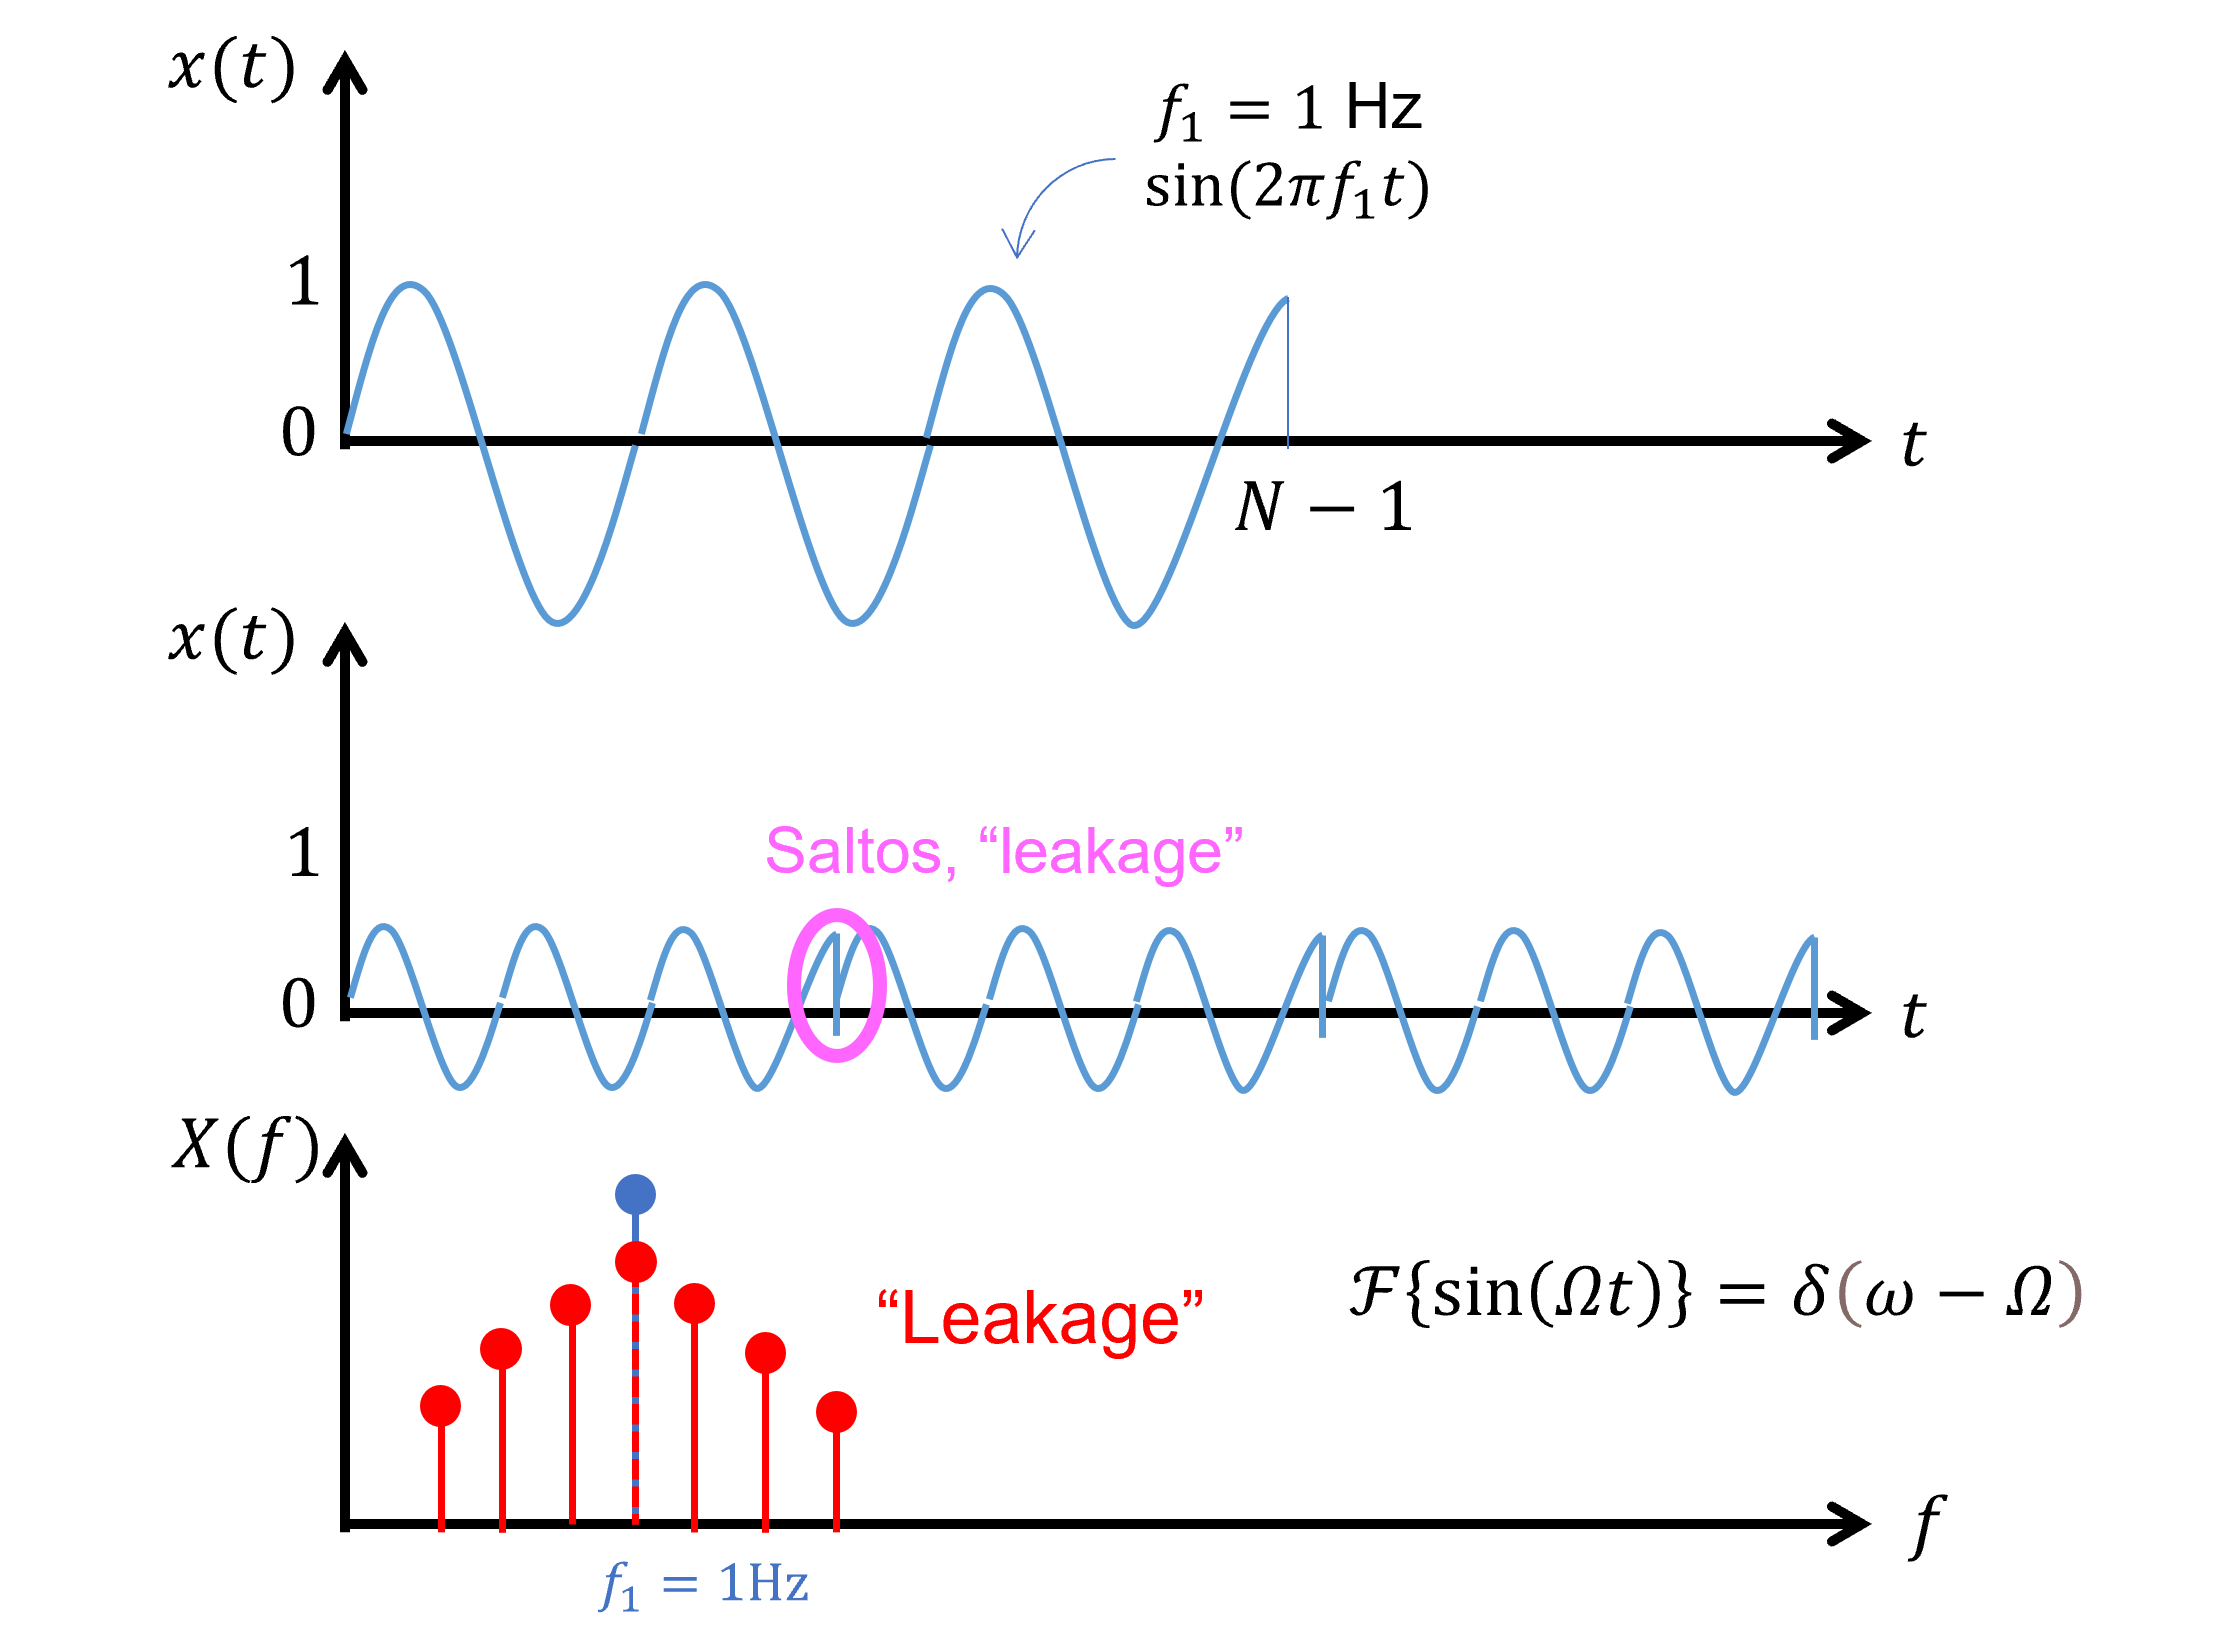
\includegraphics[width=5in]{Figuras/ejemplo_leakage.png}
\end{figure}

\par \underline{Solución}: ``Windowing'' $\Longrightarrow$ aplicar ventanas.\\

\begin{figure}[H]
    \centering
    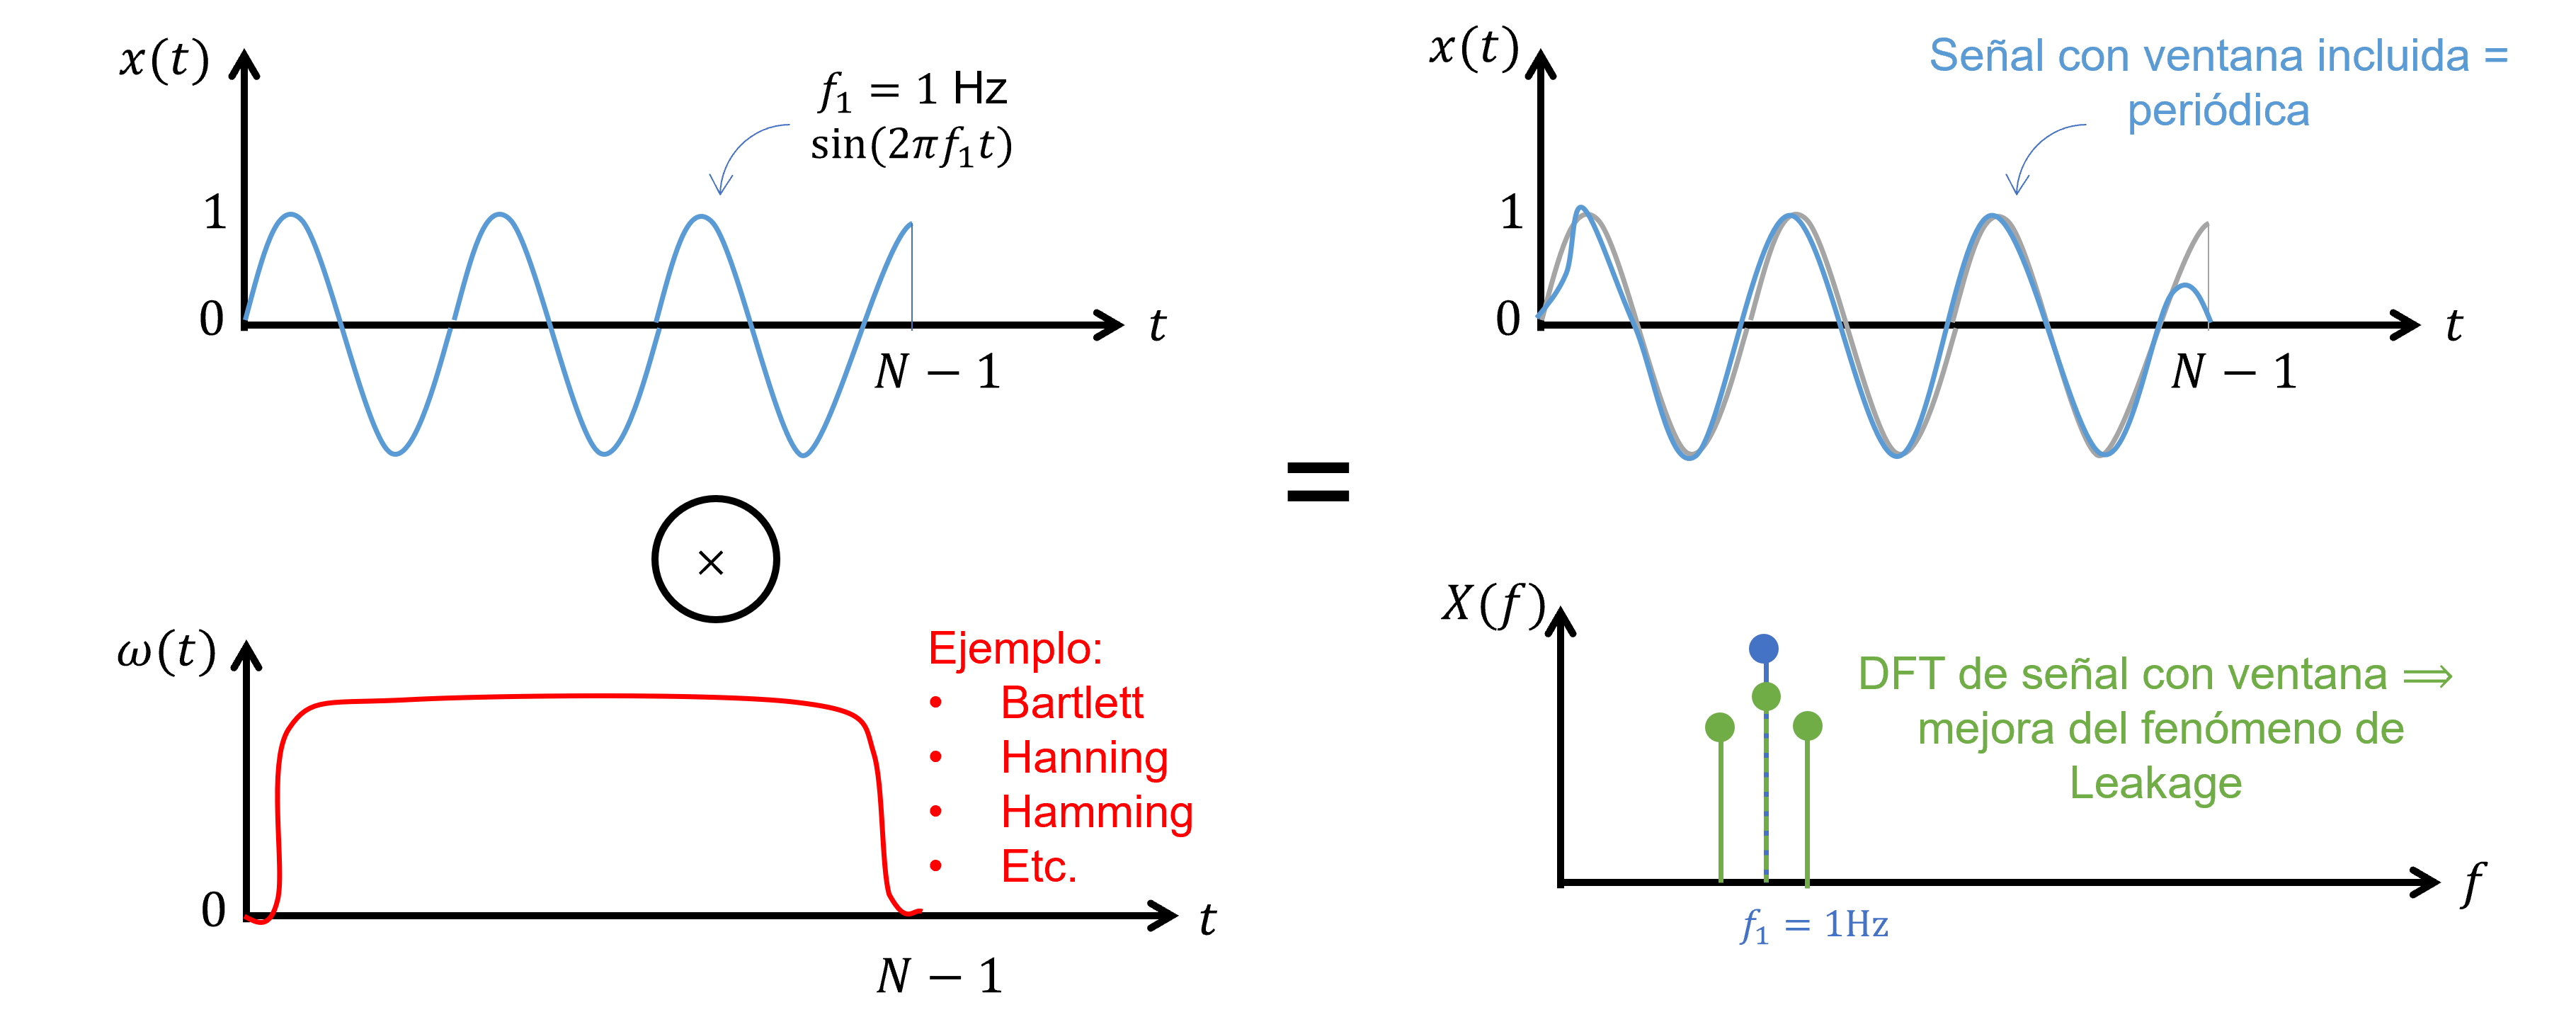
\includegraphics[width=\textwidth]{Figuras/solucion_leakage.png}
\end{figure}

También ocurre cuando la señal está contaminada con ruido. \\

Para resolver el \emph{spectral leakage} se pueden utilizar \emph{Periodogramas}.

\section{PSD de señal digital}

Referencia: \textcite[Cap. 8]{Hayes1996}.\\

En el caso de que $x(t)$ sea un p.e. w.s.s., su PSD se puede calcular de la siguiente forma:

\begin{align*}
    S_{X}(\Omega) &= \mathcal{F}\{R_{X}(\tau)\} \quad \text{(Caso contínuo, CTFT)} %\\
    %&= \mathbb{E}\{X(\omega)X^\ast(\omega)\} \quad \text{(Caso contínuo)} }
\end{align*}

En cambio, si $x[k]$ un p.e. w.s.s., señal digital con un intervalo de muestreo $T_s$. Podemos estimar $S_{X}(\omega)$ (continua) utilizando estimadores de valor medio y la definición de DTFT.

\begin{align*}
    \hat{S}_{X}(\omega) = \sum_{k=-\infty}^{+\infty}\hat{r}_x[k]e^{-j\omega k}
\end{align*}

donde el estimador de autocorrelación $\hat{r}_{X}[k]$, $n$ es el índice temporal, y $k$ es el índice para el retraso.

\begin{align*}
    \hat{r}_{X}[k] = \frac{1}{N} \sum_{n=0}^{N-1} x[n] x^*[n+k], \qquad k \in\{0,1,2,\ldots,N-1\}    
\end{align*}

\par Alcance para la estimación del PSD:

\begin{enumerate}
    \item Calcular DFT, y utilizar una forma de calcular el promedio de manera insesgada.
    \item Distintas realizaciones de $x(t)$ (de $x[k]$) nos entegan disintas estimaciones del PSD. \\ Cada estimación del PSD es una realización de un proceso estocástico.
\end{enumerate}

\begin{figure}[H]
    \centering
    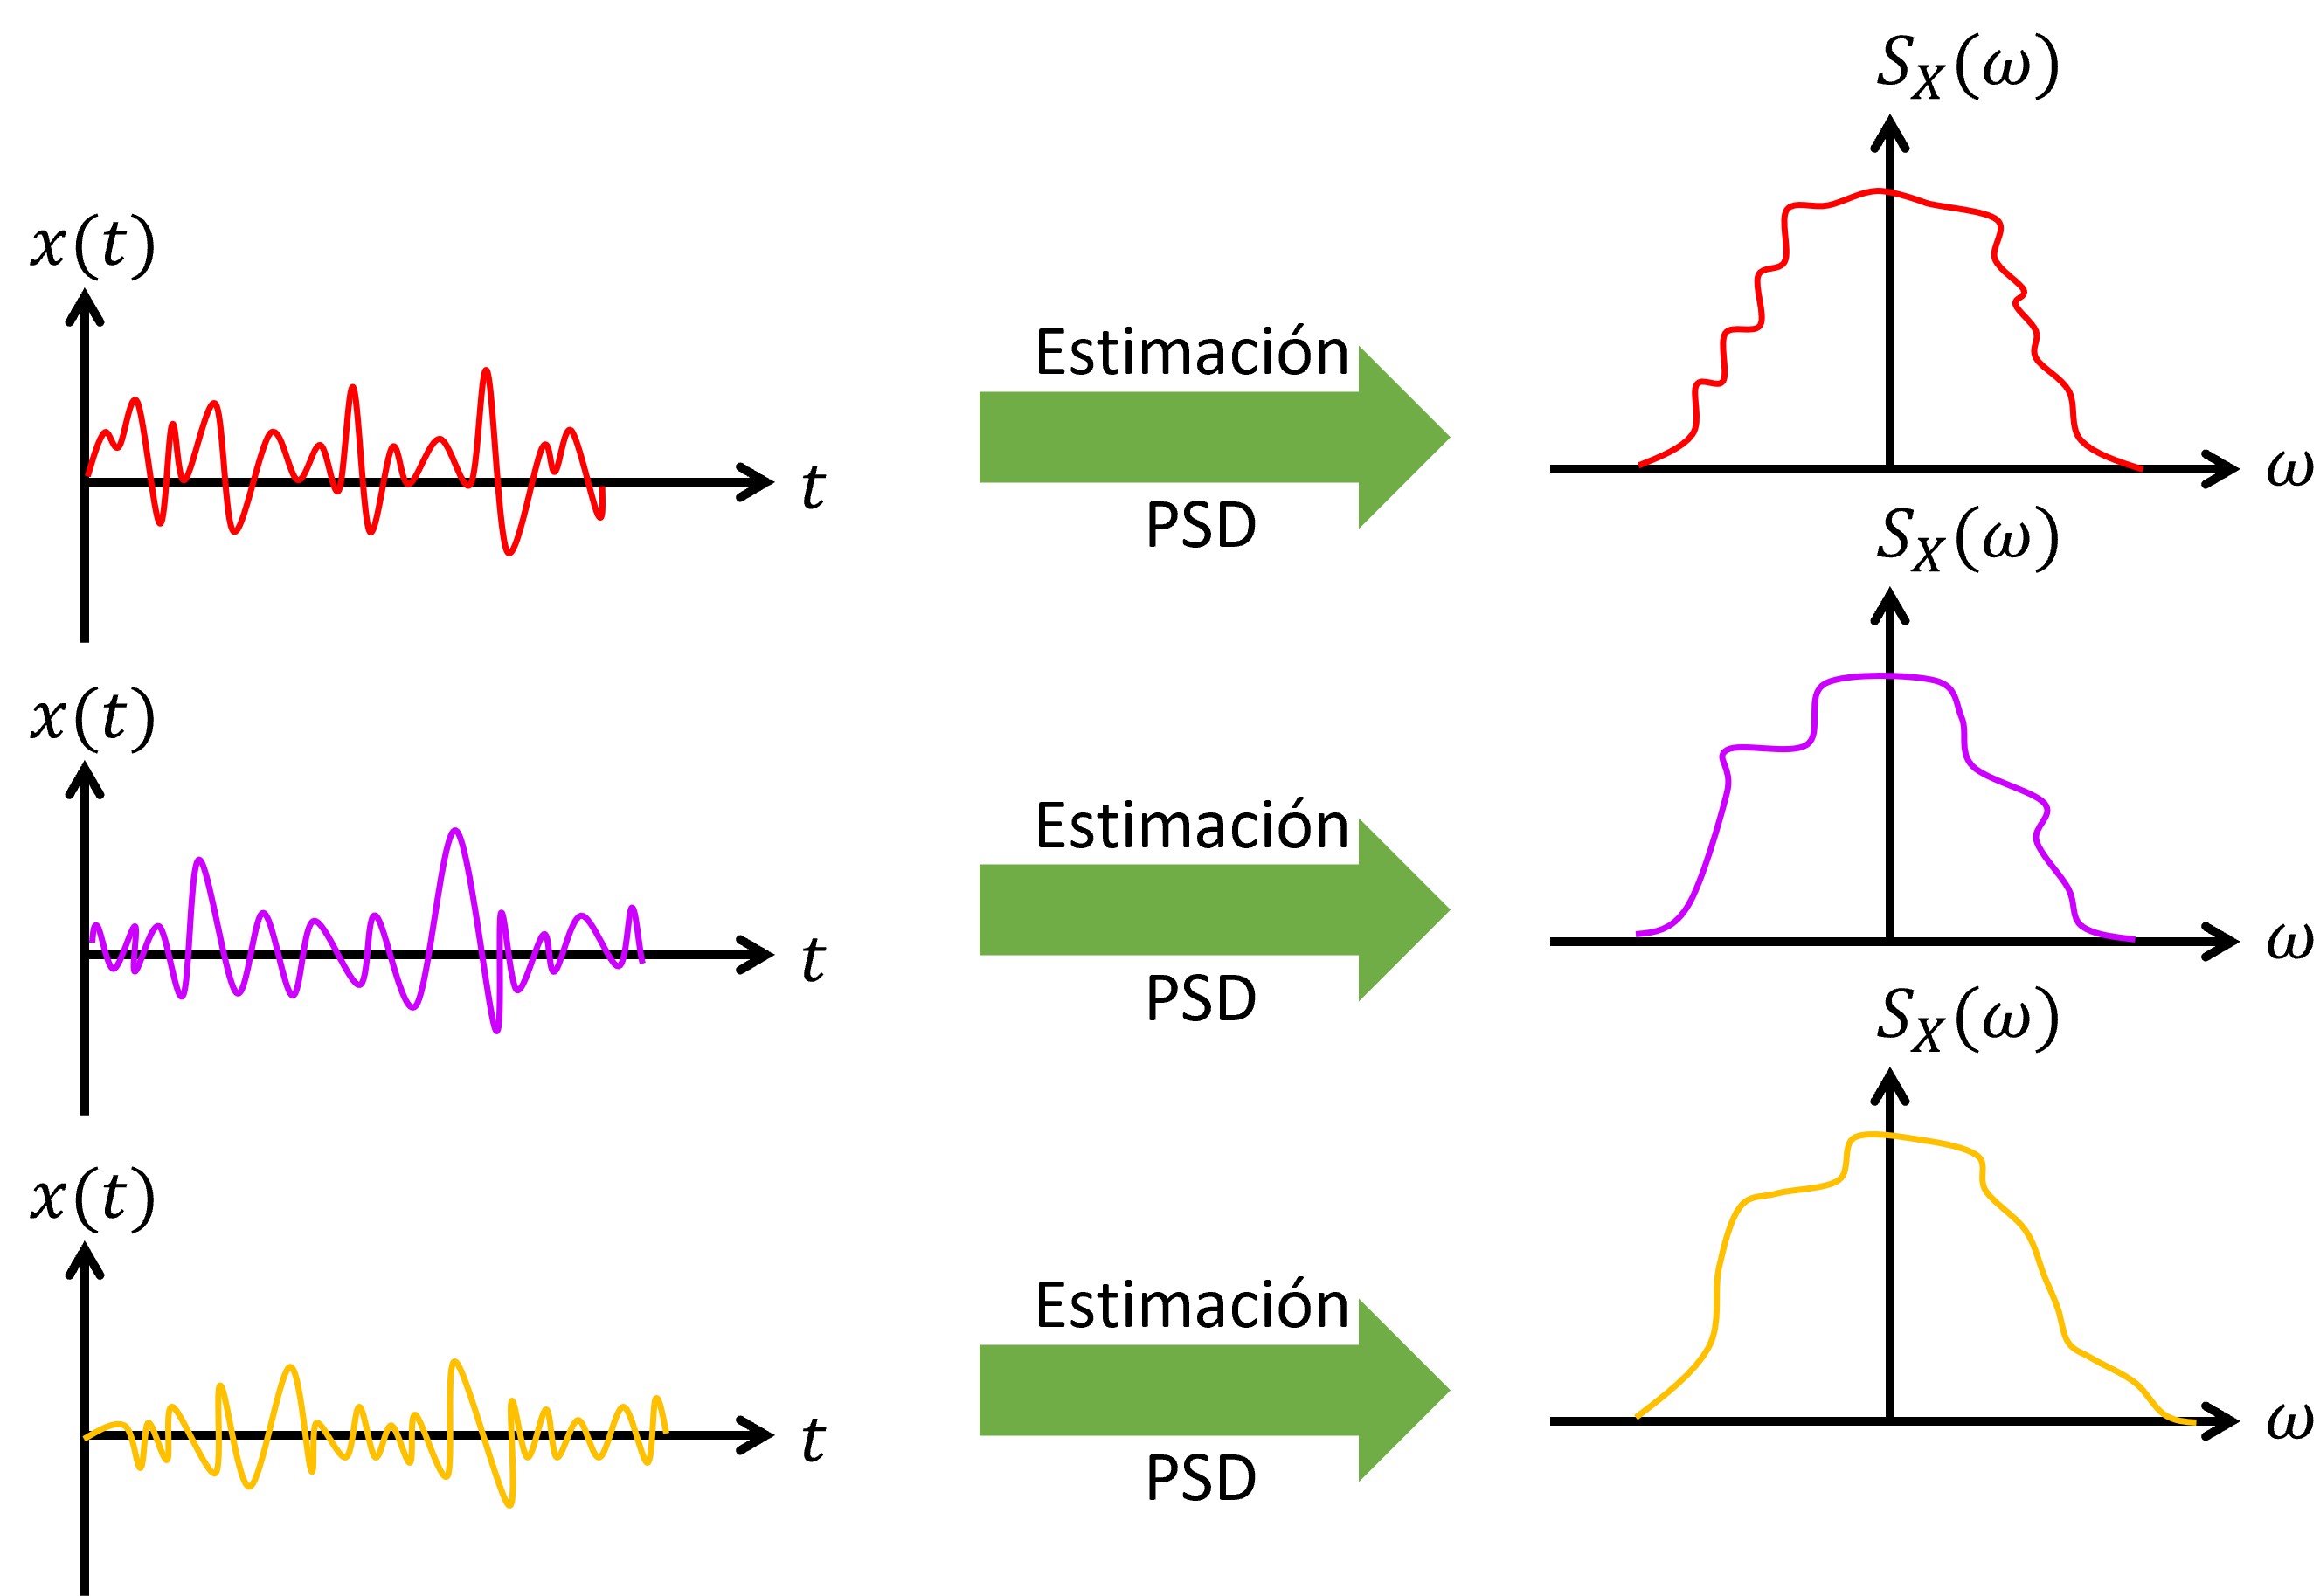
\includegraphics[scale=0.6]{Figuras/PSD_realizaciones.png}
\end{figure}

\par Estrategia para caracterizar el PSD:
\begin{enumerate}
    \item Queremos que la media del PSD se acerque al valor real del PSD.
    \item Queremos que la varianza del PSD sea pequeña.
\end{enumerate}

\underline{Ejemplo}: Considere el siguiente p.e.:
\begin{align*}
    x[n]=A+w[n]
\end{align*}

donde $A$ es una constante; $w[n] = w(nT_s)$ es ruido blanco, $\mu_W(t) = 0$ y $\sigma_W^2(t) = \sigma^2$. Entonces, $\mu_X(t) = A$ y $\sigma_X^2(t) =  \sigma^2$.\\

\par Dada una realización finita $\{x[0],x[1]...,x[N-1]\}$. Un estimador razonable para la media $A$ es la ``media muestral de A'' (promedio).

\begin{align*}
    \hat{A} = \frac{1}{N} \sum_{n=0}^{N-1}x[n]
\end{align*}

\par Entonces, queremos dos cosas:

\begin{enumerate}
    \item Que $\hat{A}$ sea insesgado, es decir, que converja al valor correcto de $A$: 
    
    $$\mathbb{E}\{\hat{A}\}=A$$
    
    Si $\hat{A}$ es sesgado. Que al menos cumpla con ser un estimador asintóticamente insesgado:
    
    $$\lim_{N\to\infty} \mathbb{E}\{\hat{A}\}=A$$
    
    \item La varianza de $\hat{A}$ sea pequeña
    
    $$\text{var}\{\hat{A}\} = \frac{\sigma^2}{N}$$ 

    En este sentido, la dispersión de $\hat{A}$ disminuye en la medida que $N$ aumenta:

    $$\lim_{N\to\infty} \text{var}\{\hat{A}\} = 0$$
    
    % \underline{Nota}: Quizás, aumentando N se disminuye la dispersión de $\hat{A}$
\end{enumerate}

\underline{Objetivos}: Estimar $\hat{S}_X(\omega)$ tal que:
$$\mathbb{E}\{\hat{S}_X(\omega)\}=S_X(\omega) $$ y 
$$\text{var}\{\hat{S}_X(\omega)\}=\text{pequeño} $$ 

\subsection{Periodograma}

\underline{Definición}: 

Usando DTFT:

\begin{align*}
    \hat{S}_{PER}(\omega) &= \frac{1}{N} \left| \sum_{n=0}^{N-1} x[n] e^{-j \omega n} \right|^2
    \\
    & = \frac{1}{N} |X(\omega)|^2\\
    & = \frac{1}{N} X(\omega) X^*(\omega)
\end{align*}

Usando DFT:

\begin{align*}
    \hat{S}_{PER}[k] &= \frac{1}{N} \left| \sum_{n=0}^{N-1} x[n] e^{-j 2 \pi n k /N} \right|^2 \\
    & = \frac{1}{N} \left| X[k] \right|^2\\
    & = \frac{1}{N} X[k] X^*[k]
\end{align*}

\underline{Nota}: 
\begin{itemize}
    % \item Considera el cálculo del DFT en vez de TF contínua
    %\item Considera un estimador neutral para el cálculo de la $\mathbb{E}\{\cdot \}$
    \item $\hat{S}_{PER}[k]$ es sesgado, pero es asintóticamente insesgado

    \begin{align*}
        \lim_{N\to\infty}\mathbb{E}\{\hat{S}_{PER}[k]\}=S_X[k]
    \end{align*}

    \item Varianza de $\hat{S}_{PER}[k]$ no tiende a cero para $N\to \infty$ $\Longrightarrow$ Problema

    \begin{align*}
        \text{var}\{\hat{S}_X(\omega)\}=\sigma^4  
    \end{align*}
    
    donde $\sigma^2=\frac{S_0 \omega_c}{\pi}$ si $x[n]$ es un ruido blanco.\\
    
\end{itemize}

Principales problemas del periodograma:

\begin{enumerate}
    \item Estimación sesgada
    \item Varianza no decrece con aumento $N$
    \item Fluctuaciones rápidas
    \begin{figure}[H]
    \centering
    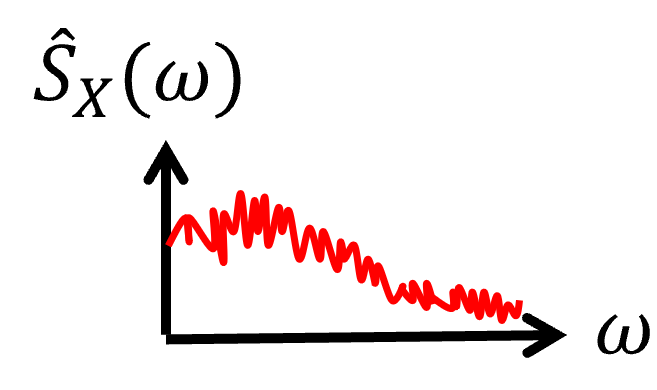
\includegraphics[scale=0.7]{Figuras/fluct.png}
    \end{figure}
\end{enumerate}

\subsection{Periodograma Modificado}

Métodos que modifican el periodograma clásico, para resolver los problemas estacionarios:

\begin{itemize}
    \item \underline{Periodograma modificada}: uso de ventanas, que reduce el efecto del sesgo, pero sacrificando resolución.
    
    $$\hat{S}_{MP}(\omega)=\frac{1}{N U} \left| \sum_{n=0}^{N-1} x[n]w[n]e^{-j\omega n} \right| ^2 $$
    
    donde $w[n]$: ventana en el dominio del tiempo y $U$ es un factor de escala.
    
    $$U=\frac{1}{N}\sum_{n=0}^{N-1}  w[n]^2$$

    Nota: $U=1$ si la ventana es rectangular.

    Desempeño:

    \begin{itemize}
        \item Reduce sesgo, pero sigue siendo una estimación sesgada.
        \item Es asintóticamente insesgada.
        \item La varianza es bastante cercana a la del periodograma.
    \end{itemize}
    
    \item \underline{Método de Bartlett}: promedio de periodogramas). Dividir la señal en $K$ segmentos de $L$ muestras, tal que $N = KL$.
    
    \begin{figure}[H]
        \centering
        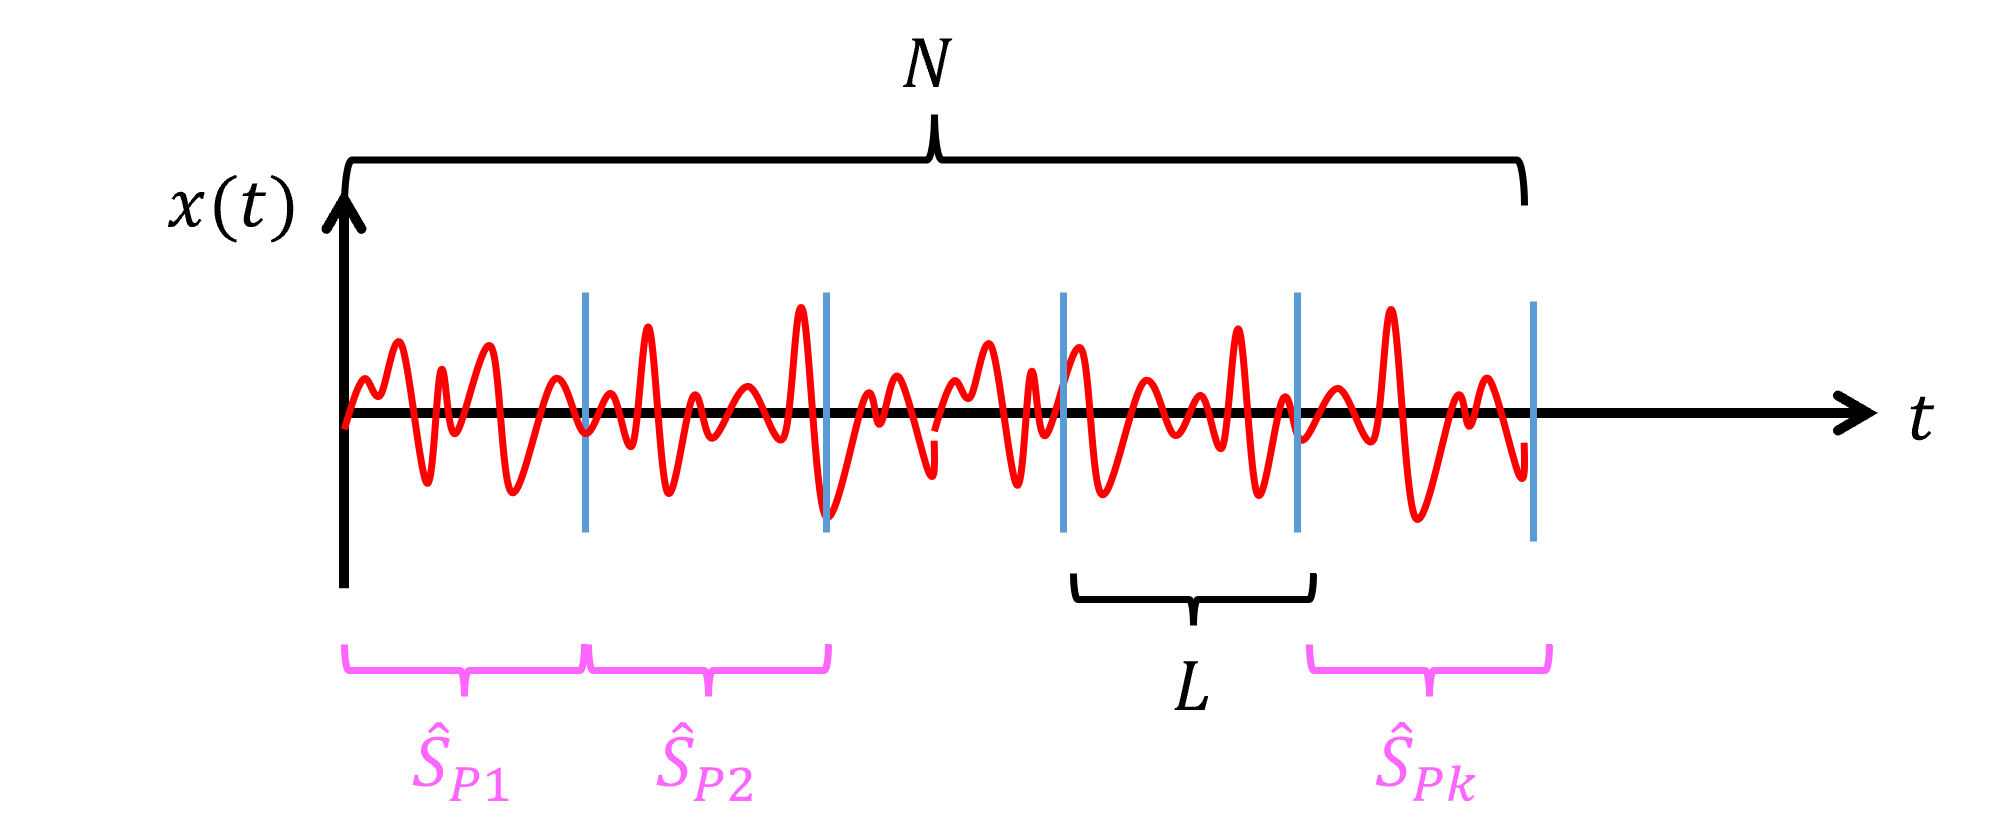
\includegraphics[scale=0.7]{Figuras/ventana1.png}
    \end{figure}

    Definición de bloque:

    $$
    x_i[n] = x[n + iL], \qquad
    \begin{cases}
        n &= \{0,1,\ldots,L-1\} \\
        i &= \{0,1,\ldots,K-1\}
    \end{cases}
    $$

    Entonces, la estimación del PSD es:
    
    $$\hat{S}_B(\omega)=\frac{1}{K}\sum_{i=0}^{K-1} \left\{\frac{1}{L} \left|\sum_{n=0}^{L-1}x_i[n]e^{-j\omega n} \right|^2 \right\} $$
    
    donde $i$ esta asociado al bloque $i$ de tamaño $L$.

    La varianza de la estimación del PSD es inversamente proporcional a la cantidad de bloques $K$:
    
    $$\text{var}\{\hat{S}_B(\omega)\} \propto \frac{1}{K}$$
    
    Es decir, que mientras más bloques se escogan (mayor $K$) más nos acercamos al objetivo de que la varianza sea $0$. \\
    
    El problema es que como $N = KL$, si se definen más bloques (aumentar $K$), significa que los bloques son más cortos ($L$ disminuye) y bloques cortos implican una resolución en frecuencia baja, es decir, $\Delta \omega$ es grande.
    
   % $$X[k] = \sum_{n=0}^{L-1}x[n]e^{-j2\pi nk/L} \quad \text{(DFT)}$$
    
    $\Longrightarrow$ ``Trade-off'': Varianza vs resolución.
    
    \item \underline{Método de Welch}: promedio de periodogramas con ventanas traslapadas.
    
    \begin{figure}[H]
        \centering
        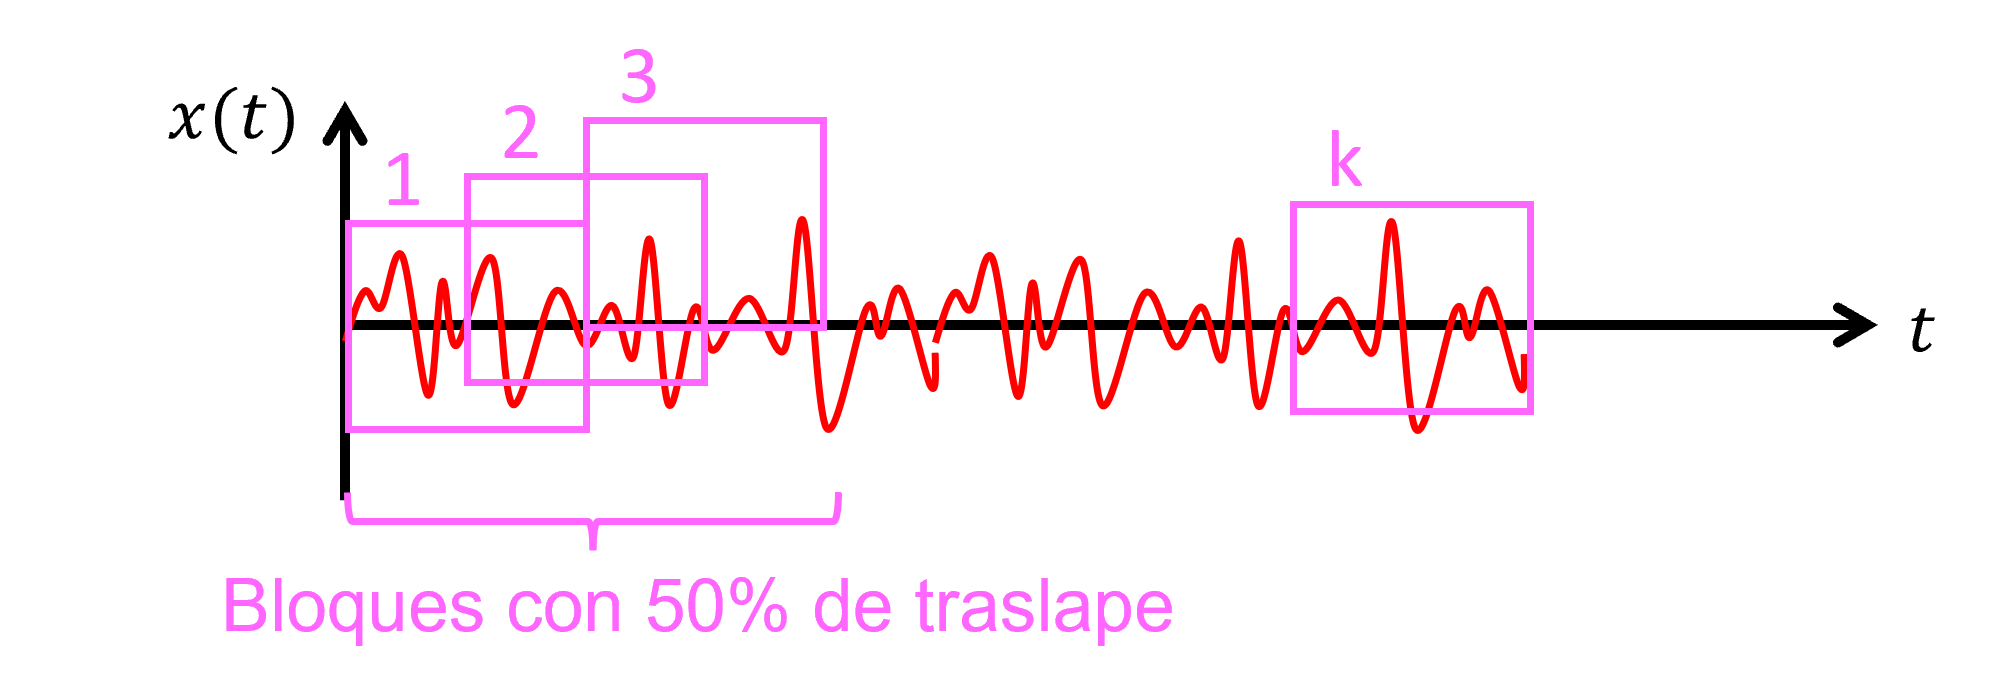
\includegraphics[scale=0.7]{Figuras/ventana2.png}
    \end{figure}

    Definición de bloque:

    $$
    x_i[n] = x[n + iD], \qquad
    \begin{cases}
        n &= \{0,1,\ldots,L-1\} \\
        i &= \{0,1,\ldots,K-1\}
    \end{cases}
    $$

    donde la cantidad de puntos de traslape es $L-D$:

    $$
    \begin{cases}
        D = L, & \text{sin traslape} \\
        D = L/2, & \text{50\% traslape (más común)}\\
        D = 3L/4, & \text{25\% traslape}
    \end{cases}
    $$
    
    $$\hat{S}_W (\omega) =\frac{1}{KLU}\sum_{i=0}^{K-1}\left| \sum_{n=0}^{L-1} x_i[n]w[n]e^{-j\omega n} \right|^2$$

    % La varianza de la estimación del PSD es inversamente proporcional a la cantidad de bloques $K$:
    
    % $$\text{var}\{\hat{S}_W (\omega)\} \approx \frac{9}{16}\frac{L}{N} S_X(\omega)^2 $$

    Comparado con método de Bartlett (sin traslape), para el mismo valor de $N$ y $L$, el método de Welch arroja casi un 50\% de reducción en varianza:

      $$\text{var}\{\hat{S}_W (\omega)\} \approx \frac{9}{16} \text{var}\{\hat{S}_B (\omega)\} $$
    
    En \emph{MATLAB}, la función \texttt{cpsd()} y \texttt{pwelch()} utilizan el método de Welch.
    
    % \item \underline{Método de Blackman-Tukey}:

    % \emph{(En desarrollo)}

    % En \emph{MATLAB}, la función \texttt{spa()} utiliza el método de Blackman-Tukey. Link: \url{https://www.mathworks.com/help/ident/ref/spa.html}.
    
\end{itemize}